\chapter[Metodologia]{Metodologia}

\section{Classificação da pesquisa}
A classificação da metodologia de pesquisa depende de diversos aspectos, tais como natureza, objetivos, abordagem e procedimentos \citeonline{gerhardt_metodos_nodate}. No presente estudo, a pesquisa é considerada como básica, focando na geração de novos conhecimentos para o avanço da ciência, sem uma aplicação prática imediata. Seu objetivo principal é explorar verdades e interesses universais, ampliando o entendimento em uma área específica do conhecimento \citeonline{prodanov_2013}.

A pesquisa em questão é classificada como descritiva em termos de objetivos. Nessa abordagem, o pesquisador se dedica a registrar e descrever os fatos observados, evitando qualquer interferência neles. A pesquisa descritiva tem como propósito principal a descrição das características de uma população ou fenômeno específico, estabelecendo também relações entre as variáveis envolvidas. Geralmente, essa modalidade de pesquisa adota uma abordagem de levantamento, em que os dados são coletados, registrados, analisados e organizados sem qualquer manipulação por parte do pesquisador. Seu objetivo é descobrir a frequência de ocorrência de um determinado fato, suas características, causas e suas relações com outros elementos \citeonline{prodanov_2013}.

No que diz respeito à abordagem, a pesquisa é considerada quantitativa. Nessa perspectiva, busca-se quantificar as informações coletadas, traduzindo opiniões e dados em números para classificação e análise. Recursos e técnicas estatísticas, como porcentagem, média, moda, mediana, desvio padrão, coeficiente de correlação e análise de regressão, são empregados para analisar os dados coletados. A pesquisa quantitativa tem como objetivo mensurar as variáveis em estudo, permitindo uma análise estatística dos resultados \citeonline{prodanov_2013}.

Quanto aos procedimentos, a pesquisa é caracterizada como experimental. Nesse tipo de abordagem, seleciona-se um objeto de estudo e identificam-se as variáveis que podem influenciá-lo. Em seguida, são estabelecidas formas de controle e observação dos efeitos que essas variáveis têm sobre o objeto em questão. O objetivo é demonstrar o modo ou as causas pelas quais um fato é produzido, possibilitando o estudo das suas relações de causa e efeito \citeonline{prodanov_2013}.

\section{Ferramentas}
As ferramentas utilizadas como suporte para a realização deste trabalho estão registradas na Tabela \ref{tab:ferramentas}.

\begin{table}[H]
\begin{tabular}{|l|l|}
\hline
\multicolumn{1}{|c|}{\textbf{Ferramenta}} & \multicolumn{1}{c|}{\textbf{Descrição}}                                                                                                                                                                 \\ \hline
Overleaf                                  & \begin{tabular}[c]{@{}l@{}}Plataforma online que permite a edição, colaboração e compilação de \\ documentos em LaTeX de forma fácil e prática.\end{tabular}                                            \\ \hline
Microsoft Teams                           & \begin{tabular}[c]{@{}l@{}}Plataforma de comunicação que permite a troca de mensagens, \\ videochamadas, compartilhamento de arquivos e trabalho em equipe \\ de forma integrada.\end{tabular}          \\ \hline
Zotero                                    & \begin{tabular}[c]{@{}l@{}}Software de gerenciamento de referências bibliográficas que facilita a \\ organização, citação e criação de bibliografias em trabalhos acadêmicos.\end{tabular}              \\ \hline
Miro                                      & \begin{tabular}[c]{@{}l@{}}Plataforma colaborativa online que permite a criação de diagramas \\ utilizada para criar o BPMN.\end{tabular}                                                               \\ \hline
Planilhas Google                          & \begin{tabular}[c]{@{}l@{}}Ferramenta de planilhas online que permite criar, editar e compartilhar \\ documentos de planilhas de forma colaborativa, utilizada para criar o \\ cronograma.\end{tabular} \\ \hline
SPSS                                      & \begin{tabular}[c]{@{}l@{}}Software de análise estatística utilizado para realizar análises de dados, \\ gerar relatórios e visualizações estatísticas.\end{tabular}                                    \\ \hline
\end{tabular}
    \caption{Ferramentas utilizadas.\\
    Fonte: Autores.}
\label{tab:ferramentas}
\end{table}

\section{Fonte de Dados: TIC Domicílios}

\subsection{O que é o TIC Domicílios}
O TIC Domicílios é uma pesquisa realizada anualmente desde 2005 pelo Centro Regional de Estudos para o Desenvolvimento da Sociedade da Informação (Cetic.br), um departamento do Núcleo de Informação e Coordenação do Ponto BR (NIC.br) \cite{ribeiro_ict_2020}. O objetivo da pesquisa é registrar e analisar o acesso às Tecnologias de Informação e Comunicação (TIC) nos domicílios brasileiros, bem como as diferentes formas de uso dessas tecnologias por pessoas a partir de 10 anos de idade \cite{nicbr2020}. Os indicadores gerados pela pesquisa abordam os seguintes temas:

\begin{itemize}
    \item Acesso às TIC
    \item Uso do computador
    \item Uso da Internet
    \item Habilidades na Internet
    \item Uso do celular
    \item Governo eletrônico
    \item Comércio eletrônico
    \item Atividades culturais na Internet
\end{itemize}

\subsection{Metodologia do TIC Domicílios}
A pesquisa utiliza os domicílios e indivíduos com mais de 10 anos como unidades de análise. O \citeonline{nicbr2020} descreve que o plano amostral é baseado em informações disponibilizadas pelo Censo Demográfico e da Pesquisa Nacional por Amostra de Domicílios (PNAD) ou da Pesquisa Nacional por Amostra de Domicílios Contínua (PNADC) mais recente, conduzidas pelo Instituto Brasileiro de Geografia e Estatística (IBGE). As entrevistas são conduzidas presencialmente, tanto em áreas urbanas quanto rurais. Além disso, a amostra da pesquisa é estratificada e agrupada considerando os diversos domínios de interesse.

\subsection{Variáveis selecionadas}

As variáveis selecionadas deste estudo foram classificadas e agrupadas de acordo com suas características e subcaracterísticas de qualidade.

\subsubsection{Socioeconômicas}
\label{subsec:socio}
Foram escolhidas variáveis socioeconômicas com o propósito de identificar as características específicas dos grupos de idosos relacionadas a cada subcaracterística de qualidade de software.

\begin{longtable}{|l|l|l|}
\endfirsthead
\endhead
\hline
ID              & Descrição   \\ \hline
COD\_REGIAO\_2  & Região      \\ \hline
CLASSE\_2015    & \begin{tabular}[c]{@{}l@{}}Classe econômica \\ pelo Critério \\ Brasil 2015\end{tabular}    \\ \hline
AREA            & Área         \\ \hline
SEXO            & Sexo         \\ \hline
IDADE           & Idade        \\ \hline
FAIXA\_ETARIA   & Faixa etária  \\ \hline
GRAU\_INSTRUCAO & \begin{tabular}[c]{@{}l@{}}Grau de instrução \\ informado pelo(a) \\ respondente\end{tabular} \\ \hline
RENDA\_PESSOAL  & Renda pessoal  \\ \hline
RACA            & \begin{tabular}[c]{@{}l@{}}Cor ou raça declarada\\  pelo(a) respondente\end{tabular}         \\ \hline
\caption{Variáveis socioeconômicas selecionadas.\\
Fonte: Autores.}
\label{tabela_socioeconomica}
\end{longtable}

\subsection{Usabilidade}

\subsubsection{Operabilidade}
As seguintes variáveis foram associadas à Operabilidade, que, de acordo com as diretrizes estabelecidas pela norma \citeonline{ISO/IEC25010}, representa  a capacidade de um sistema ser utilizado pelo usuário de maneira simples e eficaz.

\begin{longtable}{|l|l|l|}
\endfirsthead
\endhead
\hline
ID          & Descrição    \\ \hline
C2\_C       & \begin{tabular}[c]{@{}l@{}}O(a) respondente nunca \\ usou a Internet por falta \\ de habilidade com o \\ computador?\end{tabular} \\ \hline
C7\_A       & \begin{tabular}[c]{@{}l@{}}Nos últimos 3 meses, \\ o(a) respondente \\ utilizou a Internet para \\ enviar e receber e-mail?\end{tabular}  \\ \hline
C7\_B       & \begin{tabular}[c]{@{}l@{}}Nos últimos 3 meses, \\ o(a) respondente \\ utilizou a Internet para \\ enviar mensagens \\ instantâneas (como, por \\ exemplo, por Facebook, \\ Skype e Whatsapp)?\end{tabular} \\ \hline
C7\_C       & \begin{tabular}[c]{@{}l@{}}Nos últimos 3 meses, o(a) \\ respondente utilizou a \\ Internet para conversar \\ por voz ou vídeo através \\ de programas como \\ Skype ou no Whatsapp?\end{tabular} \\ \hline
C7\_D1      & \begin{tabular}[c]{@{}l@{}}Nos últimos 3 meses, \\ o(a) respondente usou \\ redes sociais, como \\ Facebook, Instagram ou \\ TikTok?\end{tabular} \\ \hline
C7\_E       & \begin{tabular}[c]{@{}l@{}}Nos últimos 3 meses, \\ o(a) respondente \\ utilizou a Internet para \\ participar de listas de \\ discussão ou fóruns?\end{tabular} \\ \hline
C7\_F       & \begin{tabular}[c]{@{}l@{}}Nos últimos 3 meses, o(a) \\ respondente utilizou a \\ Internet para usar \\ microblog como, por \\ exemplo, Twitter?\end{tabular} \\ \hline
I1A\_A      & \begin{tabular}[c]{@{}l@{}}Nos últimos 3 meses, \\ o(a) respondente copiou \\ ou moveu um arquivo ou \\ uma pasta, por exemplo, \\ em um computador ou na \\ nuvem?\end{tabular}  \\ \hline
I1A\_B      & \begin{tabular}[c]{@{}l@{}}Nos últimos 3 meses, \\ o(a) respondente usou \\ ferramenta de copiar \\ e colar para duplicar ou \\ mover conteúdo, por \\ exemplo, em um \\ documento ou uma \\ mensagem?\end{tabular} \\ \hline
I1A\_C      & \begin{tabular}[c]{@{}l@{}}Nos últimos 3 meses, \\ o(a) respondente anexou \\ documento, imagem ou \\ vídeo a mensagens \\ instantâneas, e-mails ou \\ SMS?\end{tabular} \\ \hline
I1A\_D      & \begin{tabular}[c]{@{}l@{}}Nos últimos 3 meses, \\ o(a) respondente usou \\ fórmula em uma \\ planilha de cálculo?\end{tabular} \\ \hline
I1A\_E      & \begin{tabular}[c]{@{}l@{}}Nos últimos 3 meses, \\ o(a) respondente \\ conectou ou instalou \\ novos equipamentos \\ com ou sem fio, como \\ modem, impressora, \\ câmera ou microfone?\end{tabular} \\ \hline
I1A\_F      & \begin{tabular}[c]{@{}l@{}}Nos últimos 3 meses, \\ o(a) respondente \\ instalou programas \\ de computador ou \\ aplicativos de celular?\end{tabular} \\ \hline
I1A\_G      & \begin{tabular}[c]{@{}l@{}}Nos últimos 3 meses, \\ o(a) respondente \\ criou uma apresentação \\ de slides?\end{tabular} \\ \hline
I1A\_H      & \begin{tabular}[c]{@{}l@{}}Nos últimos 3 meses, \\ o(a) respondente \\ transferiu arquivos ou \\ aplicativos entre \\ dispositivos, inclusive \\ pela nuvem?\end{tabular} \\ \hline
I1A\_I      & \begin{tabular}[c]{@{}l@{}}Nos últimos 3 meses, \\ o(a) respondente criou \\ programa de computador \\ ou aplicativo de celular \\ usando linguagem de \\ programação?\end{tabular} \\ \hline
J2\_A       & \begin{tabular}[c]{@{}l@{}}Nos últimos 3 meses, \\ o(a) respondente usou \\ o telefone celular para \\ efetuar e receber \\ chamadas telefônicas?\end{tabular} \\ \hline
J2\_B       & \begin{tabular}[c]{@{}l@{}}Nos últimos 3 meses, \\ o(a) respondente usou \\ o telefone celular para \\ enviar mensagens de \\ texto SMS?\end{tabular} \\ \hline
J2\_C       & \begin{tabular}[c]{@{}l@{}}Nos últimos 3 meses, \\ o(a) respondente usou \\ o telefone celular para \\ ouvir músicas?\end{tabular} \\ \hline
J2\_D       & \begin{tabular}[c]{@{}l@{}}Nos últimos 3 meses, \\ o(a) respondente usou \\ o telefone celular para \\ assistir vídeos?\end{tabular} \\ \hline
J2\_E       & \begin{tabular}[c]{@{}l@{}}Nos últimos 3 meses, \\ o(a) respondente usou \\ o telefone celular para \\ jogar?\end{tabular} \\ \hline
J2\_F       & \begin{tabular}[c]{@{}l@{}}Nos últimos 3 meses, \\ o(a) respondente usou \\ o telefone celular para \\ tirar fotos?\end{tabular} \\ \hline
J2\_G       & \begin{tabular}[c]{@{}l@{}}Nos últimos 3 meses, \\ o(a) respondente usou \\ o telefone celular para \\ usar mapas, por \\ exemplo o Google \\ Maps?\end{tabular} \\ \hline
J2\_H1      & \begin{tabular}[c]{@{}l@{}}Nos últimos 3 meses, \\ o(a) respondente usou \\ o telefone celular para \\ enviar e receber e-mails?\end{tabular} \\ \hline
J2\_I1      & \begin{tabular}[c]{@{}l@{}}Nos últimos 3 meses, \\ o(a) respondente usou \\ o telefone celular para \\ acessar redes sociais, \\ como Facebook, \\ Instagram ou TikTok?\end{tabular} \\ \hline
J2\_J       & \begin{tabular}[c]{@{}l@{}}Nos últimos 3 meses, \\ o(a) respondente usou \\ o telefone celular para \\ acessar páginas ou sites?\end{tabular} \\ \hline
J2\_K       & \begin{tabular}[c]{@{}l@{}}Nos últimos 3 meses, \\ o(a) respondente usou \\ o telefone celular para \\ baixar aplicativos?\end{tabular} \\ \hline
J2\_L       & \begin{tabular}[c]{@{}l@{}}Nos últimos 3 meses, \\ o(a) respondente usou \\ o telefone celular para \\ buscar informações, \\ como por exemplo no \\ Google?\end{tabular} \\ \hline
J2\_M       & \begin{tabular}[c]{@{}l@{}}Nos últimos 3 meses, \\ o(a) respondente usou \\ o telefone celular para \\ compartilhar fotos, \\ vídeos ou textos?\end{tabular} \\ \hline
J2\_N       & \begin{tabular}[c]{@{}l@{}}Nos últimos 3 meses, \\ o(a) respondente usou \\ o telefone celular para \\ enviar mensagens de \\ texto pela Internet, \\ como por WhatsApp, \\ Skype ou chat do \\ Facebook?\end{tabular} \\ \hline
G1\_A       & \begin{tabular}[c]{@{}l@{}}Nos últimos 12 meses, \\ o(a) respondente usou a \\ Internet para procurar \\ informações ou realizar \\ serviços públicos \\ relacionados a documentos \\ pessoais, como RG, CPF, \\ passaporte, ou carteira de \\ trabalho?\end{tabular} \\ \hline
G1\_B       & \begin{tabular}[c]{@{}l@{}}Nos últimos 12 meses, \\ o(a) respondente usou \\ a Internet para procurar \\ informações ou realizar \\ serviços públicos \\ relacionados a saúde \\ pública, como \\ agendamento de consultas, \\ remédios ou outros serviços \\ do sistema público de saúde?\end{tabular} \\ \hline
G1\_C       & \begin{tabular}[c]{@{}l@{}}Nos últimos 12 meses, \\ o(a) respondente usou a \\ Internet para procurar \\ informações ou realizar \\ serviços públicos \\ relacionados a educação \\ pública, como ENEM, \\ Prouni, matrícula em \\ escolas ou universidades \\ públicas?\end{tabular} \\ \hline
G1\_D       & \begin{tabular}[c]{@{}l@{}}Nos últimos 12 meses, \\ o(a) respondente usou a \\ Internet para procurar \\ informações ou realizar \\ serviços públicos \\ relacionados a direitos \\ do trabalhador ou \\ previdência social, como \\ INSS, FGTS, \\ seguro-desemprego, \\ auxílio-doença, ou \\ aposentadoria?\end{tabular} \\ \hline
G1\_E       & \begin{tabular}[c]{@{}l@{}}Nos últimos 12 meses, \\ o(a) respondente usou a \\ Internet para procurar \\ informações ou realizar \\ serviços públicos \\ relacionados a impostos \\ e taxas governamentais, \\ como declaração de \\ imposto de renda, IPVA, \\ ou IPTU?\end{tabular} \\ \hline
G1\_F       & \begin{tabular}[c]{@{}l@{}}Nos últimos 12 meses, \\ o(a) respondente usou a \\ Internet para procurar \\ informações ou realizar \\ serviços públicos \\ relacionados a polícia e \\ segurança como boletim \\ de ocorrência, \\ antecedentes criminais \\ ou denúncias?\end{tabular} \\ \hline
G1\_G       & \begin{tabular}[c]{@{}l@{}}Nos últimos 12 meses, \\ o(a) respondente usou a \\ Internet para procurar \\ informações ou realizar \\ serviços públicos \\ relacionados a transporte \\ público ou outros serviços \\ urbanos, como limpeza e \\ conservação de vias, \\ iluminação?\end{tabular} \\ \hline
C1\_COB\_A  & \begin{tabular}[c]{@{}l@{}}O(a) respondente já enviou \\ ou recebeu e-mails?\end{tabular} \\ \hline
C1\_COB\_B  & \begin{tabular}[c]{@{}l@{}}O(a) respondente já mandou \\ mensagens por WhatsApp \\ ou Telegram?\end{tabular} \\ \hline
C1\_COB\_C1 & \begin{tabular}[c]{@{}l@{}}O(a) respondente já usou \\ redes sociais como \\ Facebook ou TikTok?\end{tabular} \\ \hline
C1\_COB\_D  & \begin{tabular}[c]{@{}l@{}}O(a) respondente já buscou \\ informações no Google \\ ou Bing?\end{tabular} \\ \hline
\caption{Variáveis selecionadas associadas à característica Usabilidade e à \\subcaracterística Operabilidade.\\
Fonte: Autores.}
\label{usabilidade_operabilidade_variaveis}
\end{longtable}

\subsubsection{Aprendibilidade}
As seguintes variáveis foram associadas à Aprendibilidade, que, de acordo com as diretrizes estabelecidas pela norma \citeonline{ISO/IEC25010}, representa a capacidade em que a utilização do sistema pode ser aprendida
pelo usuário.
\begin{longtable}{|l|l|l|}
\endfirsthead
\endhead
\hline
ID              & Descrição \\ \hline
C7\_A       & \begin{tabular}[c]{@{}l@{}}Nos últimos 3 meses, \\ o(a) respondente \\ utilizou a Internet para \\ enviar e receber e-mail?\end{tabular} \\ \hline
C7\_B       & \begin{tabular}[c]{@{}l@{}}Nos últimos 3 meses, \\ o(a) respondente \\ utilizou a Internet para \\ enviar mensagens \\ instantâneas (como, por \\ exemplo, por Facebook, \\ Skype e Whatsapp)?\end{tabular} \\ \hline
C7\_C       & \begin{tabular}[c]{@{}l@{}}Nos últimos 3 meses, o(a) \\ respondente utilizou a \\ Internet para conversar \\ por voz ou vídeo através \\ de programas como \\ Skype ou no Whatsapp?\end{tabular} \\ \hline
C7\_D1      & \begin{tabular}[c]{@{}l@{}}Nos últimos 3 meses, \\ o(a) respondente usou \\ redes sociais, como \\ Facebook, Instagram ou \\ TikTok?\end{tabular} \\ \hline
C7\_E       & \begin{tabular}[c]{@{}l@{}}Nos últimos 3 meses, \\ o(a) respondente \\ utilizou a Internet para \\ participar de listas de \\ discussão ou fóruns?\end{tabular} \\ \hline
C7\_F       & \begin{tabular}[c]{@{}l@{}}Nos últimos 3 meses, o(a) \\ respondente utilizou a \\ Internet para usar \\ microblog como, por \\ exemplo, Twitter?\end{tabular} \\ \hline
H3\_D1 & \begin{tabular}[c]{@{}l@{}}Por quais dos seguintes motivos \\ o(a) respondente não comprou \\ ou encomendou produtos ou \\ serviços pela Internet nos \\ últimos 12 meses? Por falta de \\ habilidade com a Internet\end{tabular} \\ \hline
\caption{Variáveis selecionadas associadas à característica Usabilidade e à subcaracterística Aprendibilidade.\\
Fonte: Autores.}
\label{usabilidade_aprendibilidade_variaveis}
\end{longtable}


\subsubsection{Acessibilidade}
As seguintes variáveis foram associadas à Acessibilidade, que, de acordo com as diretrizes estabelecidas pela norma \citeonline{ISO/IEC25010}, representa a capacidade de um sistema de ser usado por pessoas com a mais ampla gama de características e habilidades.

\begin{longtable}{|l|l|l|}
\endfirsthead
\endhead

\hline
ID              & Descrição \\ \hline
C7\_A       & \begin{tabular}[c]{@{}l@{}}Nos últimos 3 meses, \\ o(a) respondente \\ utilizou a Internet para \\ enviar e receber e-mail?\end{tabular} \\ \hline
C7\_B       & \begin{tabular}[c]{@{}l@{}}Nos últimos 3 meses, \\ o(a) respondente \\ utilizou a Internet para \\ enviar mensagens \\ instantâneas (como, por \\ exemplo, por Facebook, \\ Skype e Whatsapp)?\end{tabular} \\ \hline
C7\_C       & \begin{tabular}[c]{@{}l@{}}Nos últimos 3 meses, o(a) \\ respondente utilizou a \\ Internet para conversar \\ por voz ou vídeo através \\ de programas como \\ Skype ou no Whatsapp?\end{tabular} \\ \hline
C7\_D1      & \begin{tabular}[c]{@{}l@{}}Nos últimos 3 meses, \\ o(a) respondente usou \\ redes sociais, como \\ Facebook, Instagram ou \\ TikTok?\end{tabular} \\ \hline
C7\_E       & \begin{tabular}[c]{@{}l@{}}Nos últimos 3 meses, \\ o(a) respondente \\ utilizou a Internet para \\ participar de listas de \\ discussão ou fóruns?\end{tabular} \\ \hline
C7\_F       & \begin{tabular}[c]{@{}l@{}}Nos últimos 3 meses, o(a) \\ respondente utilizou a \\ Internet para usar \\ microblog como, por \\ exemplo, Twitter?\end{tabular} \\ \hline
\caption{Variáveis selecionadas associadas à característica Usabilidade e à subcaracterística Acessibilidade.\\
Fonte: Autores.}
\label{usabilidade_acessibilidade_variaveis}
\end{longtable}

\subsubsection{Reconhecimento de Adequação}
A seguinte variável foi associada ao Reconhecimento de Adequação, que, de acordo com as diretrizes estabelecidas pela norma \citeonline{ISO/IEC25010}, representa a capacidade de um sistema de ser avaliado, de forma que o usuário possa reconhecer se ele está adequado para as suas necessidades.
\begin{table}[H]
\begin{tabular}{|l|l|l|}
\hline
ID    & Descrição \\ \hline
C2\_B & \begin{tabular}[c]{@{}l@{}}O(a) respondente nunca \\ usou a Internet por falta \\ de interesse?\end{tabular} \\ \hline
\end{tabular}
\caption{Variáveis selecionadas associadas à característica Usabilidade e à subcaracterística Reconhecimento de Adequação.\\
Fonte: Autores.}
\label{usabilidade_adequacao_variaveis}
\end{table}


\subsection{Segurança}

\subsubsection{Autenticidade}
As seguintes variáveis foram associadas à Autenticidade, que, de acordo com as diretrizes estabelecidas pela norma \citeonline{ISO/IEC25010}, representa a capacidade de um sistema de determinar se a identidade de um recurso ou sujeito é igual à reinvidicada.

\begin{table}[H]
\begin{tabular}{|l|l|l|}
\hline
ID     & Descrição \\ \hline
C2\_F  & \begin{tabular}[c]{@{}l@{}}O(a) respondente nunca usou \\ a Internet por preocupações \\ com segurança ou privacidade?\end{tabular} \\ \hline
I1A\_J & \begin{tabular}[c]{@{}l@{}}Nos últimos 3 meses, \\ o(a) respondente adotou \\ medidas de segurança, \\ como senhas fortes ou \\ verificação em duas etapas, \\ para proteger dispositivos \\ e contas online?\end{tabular} \\ \hline
\end{tabular}
\caption{Variáveis selecionadas associadas à característica Segurança e à subcaracterística Autenticidade.\\
Fonte: Autores.}
\label{seguranca_autenticidade_variaveis}
\end{table}

\subsubsection{Confidencialidade}
As seguintes variáveis foram associadas à Confidencialidade, que, de acordo com as diretrizes estabelecidas pela norma \citeonline{ISO/IEC25010}, representa a capacidade de um sistema de restringir o acesso a dados apenas para pessoas que tenham acesso autorizado.
\begin{table}[H]
\begin{tabular}{|l|l|l|}
\hline
ID     & Descrição \\ \hline
C2\_G  & \begin{tabular}[c]{@{}l@{}}O(a) respondente nunca usou \\ a Internet para evitar o contato \\ com conteúdo perigoso?\end{tabular} \\ \hline
H3\_F1 & \begin{tabular}[c]{@{}l@{}}Por quais dos seguintes motivos o(a) \\ respondente não comprou ou \\ encomendou produtos ou serviços \\ pela Internet nos últimos 12 meses? \\ Por ter preocupação em fornecer \\ informações pessoais\end{tabular} \\ \hline
I1A\_K & \begin{tabular}[c]{@{}l@{}}Nos últimos 3 meses, o(a) respondente \\ mudou configurações de privacidade no \\ seu dispositivo, conta ou aplicativo para \\ limitar o compartilhamento de dados \\ pessoais, como seu nome, contato ou \\ foto?\end{tabular} \\ \hline
\end{tabular}
\caption{Variáveis selecionadas associadas à característica Segurança e à subcaracterística Confidencialidade.\\
Fonte: Autores.}
\label{seguranca_autenticidade_variaveis}
\end{table}

\subsection{Portabilidade}

\subsubsection{Adaptabilidade}
As seguintes variáveis foram associadas à Adaptabilidade, que, de acordo com as diretrizes estabelecidas pela norma \citeonline{ISO/IEC25010}, representa a capacidade de um sistema de ser efetiva e eficientemente adaptado para diferentes hardwares e ambientes.

\begin{longtable}{|l|l|l|}
\endfirsthead
\endhead
\hline
ID        & Descrição \\ \hline
C5\_A     & \begin{tabular}[c]{@{}l@{}}Nos últimos 3 meses, \\ o(a) respondente utilizou \\ a Internet no computador \\ de mesa?\end{tabular} \\ \hline
C5\_B     & \begin{tabular}[c]{@{}l@{}}Nos últimos 3 meses, \\ o(a) respondente utilizou \\ a Internet no notebook?\end{tabular} \\ \hline
C5\_C     & \begin{tabular}[c]{@{}l@{}}Nos últimos 3 meses, \\ o(a) respondente utilizou \\ a Internet no tablet?\end{tabular} \\ \hline
C5\_D     & \begin{tabular}[c]{@{}l@{}}Nos últimos 3 meses, \\ o(a) respondente utilizou \\ a Internet no telefone celular?\end{tabular} \\ \hline
C5\_E     & \begin{tabular}[c]{@{}l@{}}Nos últimos 3 meses, \\ o(a) respondente utilizou \\ a Internet no videogame?\end{tabular} \\ \hline
C5\_F     & \begin{tabular}[c]{@{}l@{}}Nos últimos 3 meses, \\ o(a) respondente utilizou \\ a Internet na televisão?\end{tabular} \\ \hline
C5\_OUTRO & \begin{tabular}[c]{@{}l@{}}Nos últimos 3 meses, \\ o(a) respondente utilizou \\ a Internet em outro aparelho?\end{tabular} \\ \hline
B1        & \begin{tabular}[c]{@{}l@{}}O(a) respondente já usou um \\ computador de mesa, um \\ notebook ou um tablet?\end{tabular} \\ \hline
B4\_A     & \begin{tabular}[c]{@{}l@{}}Nos últimos 3 meses, \\ o(a) respondente usou \\ um computador de mesa, \\ um notebook ou um tablet \\ em casa?\end{tabular} \\ \hline
B4\_B     & \begin{tabular}[c]{@{}l@{}}Nos últimos 3 meses, \\ o(a) respondente usou um \\ computador de mesa, um \\ notebook ou um tablet \\ no trabalho?\end{tabular} \\ \hline
B4\_C     & \begin{tabular}[c]{@{}l@{}}Nos últimos 3 meses, \\ o(a) respondente usou um \\ computador de mesa, um \\ notebook ou um tablet na \\ escola ou estabelecimento \\ de ensino?\end{tabular} \\ \hline
B4\_D     & \begin{tabular}[c]{@{}l@{}}Nos últimos 3 meses, \\ o(a) respondente usou um \\ computador de mesa, um \\ notebook ou um tablet na \\ casa de outra pessoa, \\ como, por exemplo, \\ amigo, vizinho ou \\ familiar?\end{tabular} \\ \hline
B4\_E     & \begin{tabular}[c]{@{}l@{}}Nos últimos 3 meses, \\ o(a) respondente usou um \\ computador de mesa, um \\ notebook ou um tablet no \\ centro público de acesso \\ gratuito, como, por \\ exemplo, telecentro, \\ biblioteca ou entidade \\ comunitária?\end{tabular} \\ \hline
B4\_F     & \begin{tabular}[c]{@{}l@{}}Nos últimos 3 meses, \\ o(a) respondente usou um \\ computador de mesa, um \\ notebook ou um tablet no \\ centro público de acesso pago, \\ como, por exemplo, lanhouse, \\ cyber café ou Internet café?\end{tabular} \\ \hline
B4\_G     & \begin{tabular}[c]{@{}l@{}}Nos últimos 3 meses, \\ o(a) respondente usou um \\ computador de mesa, um \\ notebook ou um tablet \\ enquanto se desloca, como, \\ por exemplo, na rua, no \\ ônibus, no metrô ou no carro?\end{tabular} \\ \hline
B4\_H     & \begin{tabular}[c]{@{}l@{}}Nos últimos 3 meses, \\ o(a) respondente usou um \\ computador de mesa, um \\ notebook ou um tablet em \\ algum outro lugar?\end{tabular} \\ \hline
J1        & \begin{tabular}[c]{@{}l@{}}Nos últimos 3 meses, \\ o(a) respondente usou \\ um telefone celular?\end{tabular} \\ \hline
J3        & \begin{tabular}[c]{@{}l@{}}O(a) respondente usou a \\ Internet pelo telefone \\ celular nos últimos 3 meses?\end{tabular} \\ \hline
J3A\_A    & \begin{tabular}[c]{@{}l@{}}Quando o(a) respondente usou \\ a Internet pelo telefone celular \\ nos últimos 3 meses, utilizou\\ conexão 3G ou 4G?\end{tabular} \\ \hline
J3A\_B    & \begin{tabular}[c]{@{}l@{}}Quando o(a) respondente usou \\ a Internet pelo telefone celular \\ nos últimos 3 meses, utilizou \\ conexão Wi-Fi?\end{tabular} \\ \hline
J5        & \begin{tabular}[c]{@{}l@{}}O(a) respondente possui telefone \\ celular?\end{tabular} \\ \hline
\caption{Variáveis selecionadas associadas à característica Portabilidade e à subcaracterística Adaptabilidade.\\
Fonte: Autores.}
\label{portabilidade_adaptabilidade_variaveis}
\end{longtable}


\subsection{Adequação funcional}

\subsubsection{Completude Funcional}
As seguintes variáveis foram associadas à Completude Funcional, que, de acordo com as diretrizes estabelecidas pela norma \citeonline{ISO/IEC25010}, representa o grau em que um conjunto de funcionalidades atende os objetivos e tarefas do usuário.

\begin{longtable}{|l|l|l|}
\endfirsthead
\endhead
\hline
ID             & Descrição \\ \hline
C3             & \begin{tabular}[c]{@{}l@{}}Quando o(a) \\respondente usou \\ a Internet pela última \\ vez?\end{tabular} \\ \hline
C4             & \begin{tabular}[c]{@{}l@{}}Em média, com que freqüência \\ o(a) respondente usou a Internet \\ nos últimos 3 meses?\end{tabular} \\ \hline
C6\_A          & \begin{tabular}[c]{@{}l@{}}Pensando nos últimos 3 meses, \\ o(a) respondente utilizou a \\ Internet em casa?\end{tabular} \\ \hline
C6\_B          & \begin{tabular}[c]{@{}l@{}}Pensando nos últimos 3 meses, \\ o(a) respondente utilizou a \\ Internet no trabalho?\end{tabular} \\ \hline
C6\_C          & \begin{tabular}[c]{@{}l@{}}Pensando nos últimos 3 meses, \\ o(a) respondente utilizou a Internet\\ na escola ou estabelecimento de ensino?\end{tabular} \\ \hline
C6\_D          & \begin{tabular}[c]{@{}l@{}}Pensando nos últimos 3 meses, \\ o(a) respondente utilizou a Internet \\ na casa de outra pessoa, como, \\ por exemplo, amigo, vizinho ou familiar?\end{tabular} \\ \hline
C6\_E          & \begin{tabular}[c]{@{}l@{}}Pensando nos últimos 3 meses, \\ o(a) respondente utilizou a Internet \\ no centro público de acesso gratuito, \\ como, por exemplo, telecentro, \\ biblioteca ou entidade comunitária?\end{tabular} \\ \hline
C6\_F          & \begin{tabular}[c]{@{}l@{}}Pensando nos últimos 3 meses, \\ o(a) respondente utilizou a Internet \\ no centro público de acesso pago, \\ como, por exemplo, lanhouse, \\ Cyber Café ou Internet café?\end{tabular} \\ \hline
C6\_G          & \begin{tabular}[c]{@{}l@{}}Pensando nos últimos 3 meses, \\ o(a) respondente utilizou a Internet \\ enquanto se desloca, como, por \\ exemplo, na rua, no ônibus, no \\ metrô, no carro?\end{tabular} \\ \hline
C6\_OUTRO      & \begin{tabular}[c]{@{}l@{}}Pensando nos últimos 3 meses, \\ o(a) respondente utilizou a Internet\\ em outro lugar?\end{tabular}\\ \hline
C8\_A          & \begin{tabular}[c]{@{}l@{}}Nos últimos 3 meses, \\ o(a) respondente utilizou a \\ Internet para procurar \\ informações sobre produtos \\ e serviços?\end{tabular} \\ \hline
C8\_B          & \begin{tabular}[c]{@{}l@{}}Nos últimos 3 meses, \\ o(a) respondente utilizou a Internet \\ para procurar informações relacionadas \\ à saúde ou a serviços de saúde?\end{tabular} \\ \hline
C8\_C          & \begin{tabular}[c]{@{}l@{}}Nos últimos 3 meses, \\ o(a) respondente utilizou a Internet \\ para procurar informações sobre \\ viagens e acomodações?\end{tabular} \\ \hline
C8\_D          & \begin{tabular}[c]{@{}l@{}}Nos últimos 3 meses, \\ o(a) respondente utilizou \\ a Internet para procurar \\ emprego ou enviar currículos?\end{tabular} \\ \hline
C8\_E          & \begin{tabular}[c]{@{}l@{}}Nos últimos 3 meses, \\ o(a) respondente utilizou a Internet \\ para procurar informações em sites \\ de enciclopédia virtual como Wikipédia?\end{tabular} \\ \hline
C8\_F          & \begin{tabular}[c]{@{}l@{}}Nos últimos 3 meses, \\ o(a) respondente utilizou \\ a Internet para procurar \\ informações oferecidas \\ por sites de governo?\end{tabular} \\ \hline
C8\_G          & \begin{tabular}[c]{@{}l@{}}Nos últimos 3 meses, \\ o(a) respondente utilizou \\ a Internet para realizar \\ algum serviço público como, \\ por exemplo, emitir documentos \\ pela Internet, preencher e enviar \\ formulários online, ou pagar \\ taxas e impostos pela Internet?\end{tabular} \\ \hline
C8\_H          & \begin{tabular}[c]{@{}l@{}}Nos últimos 3 meses, \\ o(a) respondente utilizou \\ a Internet para fazer consultas, \\ pagamentos ou outras transações \\ financeiras?\end{tabular} \\ \hline
C9\_A          & \begin{tabular}[c]{@{}l@{}}Nos últimos 3 meses, \\ o(a) respondente utilizou \\ a Internet para jogar online?\end{tabular} \\ \hline
C9\_B          & \begin{tabular}[c]{@{}l@{}}Nos últimos 3 meses, \\ o(a) respondente utilizou \\ a Internet para ouvir música \\ online como por Spotify, por \\ Deezer ou por YouTube?\end{tabular} \\ \hline
C9\_C          & \begin{tabular}[c]{@{}l@{}}Nos últimos 3 meses, \\ o(a) respondente utilizou \\ a Internet para assistir vídeos, \\ programas, filmes ou séries em \\ sites como o YouTube ou Netflix?\end{tabular} \\ \hline
C9\_D          & \begin{tabular}[c]{@{}l@{}}Nos últimos 3 meses, \\ o(a) respondente utilizou \\ a Internet para ler jornais, \\ revistas ou notícias?\end{tabular} \\ \hline
C9\_F          & \begin{tabular}[c]{@{}l@{}}Nos últimos 3 meses, \\ o(a) respondente utilizou \\ a Internet para ver exposições \\ e museus?\end{tabular} \\ \hline
C9\_G          & \begin{tabular}[c]{@{}l@{}}Nos últimos 3 meses, \\ o(a) respondente utilizou \\ a Internet para ouvir podcasts?\end{tabular} \\ \hline
C9\_E          & \begin{tabular}[c]{@{}l@{}}Nos últimos 3 meses, \\ o(a) respondente utilizou \\ a Internet para acompanhar \\ transmissões de áudio ou \\ vídeo em tempo real ou \\ lives pela Internet?\end{tabular} \\ \hline
C10\_A         & \begin{tabular}[c]{@{}l@{}}Nos últimos 3 meses, \\ o(a) respondente utilizou \\ a Internet para realizar \\ atividades ou pesquisas \\ escolares?\end{tabular} \\ \hline
C10\_B         & \begin{tabular}[c]{@{}l@{}}Nos últimos 3 meses, \\ o(a) respondente utilizou \\ a Internet para fazer \\ cursos à distância?\end{tabular} \\ \hline
C10\_C         & \begin{tabular}[c]{@{}l@{}}Nos últimos 3 meses, \\ o(a) respondente utilizou a \\ Internet para buscar informações \\ sobre cursos de graduação, \\ pós-graduação e de extensão?\end{tabular} \\ \hline
C10\_D         & \begin{tabular}[c]{@{}l@{}}Nos últimos 3 meses, \\ o(a) respondente utilizou a \\ Internet para estudar na \\ Internet por conta própria?\end{tabular} \\ \hline
C10\_E         & \begin{tabular}[c]{@{}l@{}}Nos últimos 3 meses, \\ o(a) respondente utilizou \\ a Internet para usar serviço \\ de armazenamento na Internet, \\ como por exemplo Dropbox, \\ Google Drive, OneDrive?\end{tabular} \\ \hline
C10\_F         & \begin{tabular}[c]{@{}l@{}}Nos últimos 3 meses, \\ o(a) respondente utilizou \\ a Internet para realizar \\ atividades de trabalho?\end{tabular} \\ \hline
C11\_A         & \begin{tabular}[c]{@{}l@{}}Nos últimos 3 meses, \\ o(a) respondente utilizou \\ a Internet para compartilhar \\ conteúdo na Internet, como \\ textos, imagens, fotos, vídeos \\ ou músicas?\end{tabular} \\ \hline
C11\_B         & \begin{tabular}[c]{@{}l@{}}Nos últimos 3 meses, \\ o(a) respondente utilizou \\ a Internet para criar ou \\ atualizar blogs, páginas na \\ Internet ou websites?\end{tabular} \\ \hline
C11\_C         & \begin{tabular}[c]{@{}l@{}}Nos últimos 3 meses, \\ o(a) respondente utilizou \\ a Internet para postar na \\ Internet textos, imagens, \\ fotos, vídeos ou músicas \\ que o(a) respondente \\ mesmo fez?\end{tabular} \\ \hline
C12\_A         & \begin{tabular}[c]{@{}l@{}}Nos últimos 3 meses, \\ o(a) respondente utilizou \\ a Internet para baixar ou \\ fazer o download de filmes?\end{tabular} \\ \hline
C12\_B         & \begin{tabular}[c]{@{}l@{}}Nos últimos 3 meses, \\ o(a) respondente utilizou \\ a Internet para baixar ou \\ fazer o download de músicas?\end{tabular} \\ \hline
C12\_C         & \begin{tabular}[c]{@{}l@{}}Nos últimos 3 meses, \\ o(a) respondente utilizou \\ a Internet para baixar ou \\ fazer o download de jogos?\end{tabular} \\ \hline
C12\_D         & \begin{tabular}[c]{@{}l@{}}Nos últimos 3 meses, \\ o(a) respondente utilizou \\ a Internet para baixar ou \\ fazer o download de \\ softwares, programas de \\ computador ou aplicativos?\end{tabular} \\ \hline
C12\_E1        & \begin{tabular}[c]{@{}l@{}}Nos últimos 3 meses, \\ o(a) respondente utilizou \\ a Internet para baixar ou \\ fazer o download de livros \\ digitais?\end{tabular} \\ \hline
C12\_F1        & \begin{tabular}[c]{@{}l@{}}Nos últimos 3 meses, \\ o(a) respondente utilizou \\ a Internet para baixar ou \\ fazer o download de séries?\end{tabular} \\ \hline
H1             & \begin{tabular}[c]{@{}l@{}}Nos últimos 12 meses, \\ o(a) respondente utilizou \\ a Internet para pesquisar \\ preços de produtos ou serviços?\end{tabular} \\ \hline
H2             & \begin{tabular}[c]{@{}l@{}}Nos últimos 12 meses, \\ o(a) respondente comprou \\ ou encomendou produtos \\ ou serviços pela Internet, \\ mesmo que o pagamento \\ não tenha sido feito pela \\ Internet?\end{tabular}   \\ \hline
H3\_A1         & \begin{tabular}[c]{@{}l@{}}Por quais dos seguintes \\ motivos o(a) respondente \\ não comprou ou encomendou \\ produtos ou serviços pela \\ Internet nos últimos 12 meses? \\ Por falta de necessidade\end{tabular} \\ \hline
H5\_A          & \begin{tabular}[c]{@{}l@{}}Nos últimos 12 meses, \\ o(a) respondente comprou \\ ou encomendou pela Internet \\ comida ou produtos alimentícios?\end{tabular} \\ \hline
H5\_B          & \begin{tabular}[c]{@{}l@{}}Nos últimos 12 meses, \\ o(a) respondente comprou \\ ou encomendou pela Internet \\ produtos para a casa ou \\ eletrodomésticos?\end{tabular} \\ \hline
H5\_C          & \begin{tabular}[c]{@{}l@{}}Nos últimos 12 meses, \\ o(a) respondente comprou \\ ou encomendou pela Internet \\ roupas, calçados, material \\ esportivo?\end{tabular} \\ \hline
H5\_D          & \begin{tabular}[c]{@{}l@{}}Nos últimos 12 meses, \\ o(a) respondente comprou \\ ou encomendou pela Internet \\ equipamentos eletrônicos \\ como celulares, tablets, \\ videogames, computadores?\end{tabular} \\ \hline
H5\_F          & \begin{tabular}[c]{@{}l@{}}Nos últimos 12 meses, \\ o(a) respondente comprou \\ ou encomendou pela Internet \\ passagens aéreas?\end{tabular}  \\ \hline
H5\_G          & \begin{tabular}[c]{@{}l@{}}Nos últimos 12 meses, \\ o(a) respondente comprou \\ ou encomendou pela Internet \\ ingressos para eventos como, \\ por exemplo, shows, cinema, \\ peças de teatro, exposições, etc?\end{tabular} \\ \hline
H5\_I          & \begin{tabular}[c]{@{}l@{}}Nos últimos 12 meses, \\ o(a) respondente comprou \\ ou encomendou pela Internet \\ livros, revistas ou jornais?\end{tabular} \\ \hline
H5\_J          & \begin{tabular}[c]{@{}l@{}}Nos últimos 12 meses, \\ o(a) respondente comprou \\ ou encomendou pela Internet \\ programas de computador ou \\ aplicativos de celular?\end{tabular} \\ \hline
H5\_K          & \begin{tabular}[c]{@{}l@{}}Nos últimos 12 meses, \\ o(a) respondente comprou \\ ou encomendou pela Internet \\ jogos de computador ou de \\ videogame?\end{tabular} \\ \hline
H5\_L          & \begin{tabular}[c]{@{}l@{}}Nos últimos 12 meses, \\ o(a) respondente comprou \\ ou encomendou pela Internet \\ medicamentos?\end{tabular} \\ \hline
H5\_N          & \begin{tabular}[c]{@{}l@{}}Nos últimos 12 meses, \\ o(a) respondente comprou \\ ou encomendou pela Internet \\ cosméticos ou produtos de \\ higiene pessoal?\end{tabular} \\ \hline
H5\_O          & \begin{tabular}[c]{@{}l@{}}Nos últimos 12 meses, \\ o(a) respondente comprou \\ ou encomendou pela Internet \\ brinquedos?\end{tabular} \\ \hline
H5\_P          & \begin{tabular}[c]{@{}l@{}}Nos últimos 12 meses, \\ o(a) respondente comprou \\ ou encomendou pela Internet \\ itens de papelaria?\end{tabular} \\ \hline
H5\_OUTRO      & \begin{tabular}[c]{@{}l@{}}Nos últimos 12 meses, \\ o(a) respondente comprou \\ ou encomendou pela Internet \\ algum outro produto?\end{tabular} \\ \hline
H6             & \begin{tabular}[c]{@{}l@{}}Nos últimos 12 meses, com que \\frequência o(a) respondente comprou \\ou encomendou produtos ou serviços \\pela Internet?\end{tabular} \\ \hline
H7\_A          & \begin{tabular}[c]{@{}l@{}}Nos últimos 12 meses, \\ o(a) respondente comprou \\ ou encomendou produtos \\ ou serviços em redes sociais, \\ como, por exemplo, Facebook, \\ Instagram ou TikTok?\end{tabular} \\ \hline
H7\_B          & \begin{tabular}[c]{@{}l@{}}Nos últimos 12 meses, \\ o(a) respondente comprou \\ ou encomendou produtos \\ ou serviços por mensagens \\ instantâneas, como, por \\ exemplo, WhatsApp, \\ Skype ou Telegram?\end{tabular} \\ \hline
H7\_C          & \begin{tabular}[c]{@{}l@{}}Nos últimos 12 meses, \\ o(a) respondente comprou \\ ou encomendou produtos \\ ou serviços em sites de lojas, \\ como, por exemplo, Netshoes, \\ Submarino ou Americanas.com?\end{tabular} \\ \hline
H7\_D          & \begin{tabular}[c]{@{}l@{}}Nos últimos 12 meses, \\ o(a) respondente comprou \\ ou encomendou produtos \\ ou serviços em sites de \\ compra e venda, como \\ Mercado Livre ou OLX?\end{tabular} \\ \hline
H7\_E          & \begin{tabular}[c]{@{}l@{}}Nos últimos 12 meses, \\ o(a) respondente comprou \\ ou encomendou produtos \\ ou serviços em sites de \\ desconto como, por exemplo, \\ Peixe Urbano ou Groupon?\end{tabular} \\ \hline
H7\_F          & \begin{tabular}[c]{@{}l@{}}Nos últimos 12 meses, \\ o(a) respondente comprou \\ ou encomendou produtos \\ ou serviços por e-mail?\end{tabular} \\ \hline
H8\_A          & \begin{tabular}[c]{@{}l@{}}Nos últimos 12 meses, \\ o(a) respondente pagou por\\  esses produtos ou serviços \\ com cartão de crédito?\end{tabular} \\ \hline
H8\_B          & \begin{tabular}[c]{@{}l@{}}Nos últimos 12 meses, \\ o(a) respondente pagou por \\ esses produtos ou serviços \\ com boleto bancário?\end{tabular} \\ \hline
H8\_C          & \begin{tabular}[c]{@{}l@{}}Nos últimos 12 meses, \\ o(a) respondente pagou por \\ esses produtos ou serviços \\ com débito online ou \\ transferência bancária por \\ DOC ou TED?\end{tabular} \\ \hline
H8\_D          & \begin{tabular}[c]{@{}l@{}}Nos últimos 12 meses, \\ o(a) respondente pagou por \\ esses produtos ou serviços \\ com pagamento na entrega?\end{tabular} \\ \hline
H8\_E          & \begin{tabular}[c]{@{}l@{}}Nos últimos 12 meses, \\ o(a) respondente pagou por \\ esses produtos ou serviços \\ com serviço de pagamento \\ online, como PagSeguro, \\ PayPal ou Google Checkout?\end{tabular} \\ \hline
H8\_F          & \begin{tabular}[c]{@{}l@{}}Nos últimos 12 meses, \\ o(a) respondente pagou por \\ esses produtos ou serviços \\ com cartão de presente ou \\ voucher online?\end{tabular} \\ \hline
H8\_G          & \begin{tabular}[c]{@{}l@{}}Nos últimos 12 meses, \\ o(a) respondente pagou por \\ esses produtos ou serviços \\ com pontos de programas de \\ recompensas ou resgate?\end{tabular} \\ \hline
H8\_H          & \begin{tabular}[c]{@{}l@{}}Nos últimos 12 meses, \\ o(a) respondente pagou por \\ esses produtos ou serviços \\ com Pix?\end{tabular}   \\ \hline
H9\_A          & \begin{tabular}[c]{@{}l@{}}Nos últimos 12 meses, \\ os produtos ou serviços que \\ o(a) respondente comprou ou \\ encomendou pela Internet \\ foram entregues em casa?\end{tabular} \\ \hline
H9\_B          & \begin{tabular}[c]{@{}l@{}}Nos últimos 12 meses, \\ os produtos ou serviços que \\ o(a) respondente comprou \\ ou encomendou pela Internet \\ foram retirados na loja ou em \\ local indicado pelo vendedor?\end{tabular} \\ \hline
H9\_C          & \begin{tabular}[c]{@{}l@{}}Nos últimos 12 meses, \\ os produtos ou serviços que \\ o(a) respondente comprou ou \\ encomendou pela Internet \\ foram baixados ou acessados \\ pela Internet em sites, aplicativos \\ ou programas de computador?\end{tabular} \\ \hline
H10            & \begin{tabular}[c]{@{}l@{}}Nos últimos 12 meses, \\ somando todos os produtos \\ que comprou ou encomendou \\ pela Internet, quanto o(a) \\ respondente gastou, \\ aproximadamente?\end{tabular} \\ \hline
H11\_A         & \begin{tabular}[c]{@{}l@{}}Nos últimos 12 meses, \\ o(a) respondente comprou \\ ou encomendou algum produto \\ ou serviço pela Internet após \\ ter visto propagandas em sites \\ ou aplicativos\end{tabular}  \\ \hline
H11\_B         & \begin{tabular}[c]{@{}l@{}}Nos últimos 12 meses, \\ o(a) respondente comprou \\ ou encomendou algum produto \\ ou serviço pela Internet após \\ ter visto posts em redes sociais \\ como Facebook, Instagram ou \\ TikTok\end{tabular}  \\ \hline
H11\_C         & \begin{tabular}[c]{@{}l@{}}Nos últimos 12 meses, \\ o(a) respondente comprou \\ ou encomendou algum produto \\ ou serviço pela Internet após ter \\ visto mensagens recebidas por \\ WhatsApp, Skype ou Telegram\end{tabular} \\ \hline
H11\_D         & \begin{tabular}[c]{@{}l@{}}Nos últimos 12 meses, \\ o(a) respondente comprou \\ ou encomendou algum produto \\ ou serviço pela Internet após ter \\ visto e-mails com ofertas\end{tabular} \\ \hline
H11\_E         & \begin{tabular}[c]{@{}l@{}}Nos últimos 12 meses, \\ o(a) respondente comprou \\ ou encomendou algum produto \\ ou serviço pela Internet após ter \\ visto vídeos na Internet sobre \\ produtos ou serviços\end{tabular} \\ \hline
H12\_A         & \begin{tabular}[c]{@{}l@{}}Nos últimos 12 meses, \\ o(a) respondente pagou por \\ serviços de filmes ou séries \\ pela Internet, como, por \\ exemplo, Netflix ou Globoplay?\end{tabular} \\ \hline
H12\_B         & \begin{tabular}[c]{@{}l@{}}Nos últimos 12 meses, \\ o(a) respondente pagou por \\ serviços de músicas pela \\ Internet, como, por exemplo, \\ Spotify ou Deezer?\end{tabular} \\ \hline
H12\_C         & \begin{tabular}[c]{@{}l@{}}Nos últimos 12 meses, \\ o(a) respondente fez reservas \\ de quartos ou acomodações \\ pela Internet em sites ou \\ aplicativos, como, por \\ exemplo, Booking ou Airbnb?\end{tabular} \\ \hline
H12\_D         & \begin{tabular}[c]{@{}l@{}}Nos últimos 12 meses, \\ o(a) respondente fez \\ reserva de carro para \\ aluguel pela Internet?\end{tabular} \\ \hline
H12\_E         & \begin{tabular}[c]{@{}l@{}}Nos últimos 12 meses, \\ o(a) respondente contratou \\ serviços financeiros pela \\ Internet, como seguros, \\ empréstimos ou financiamentos?\end{tabular} \\ \hline
H12\_F         & \begin{tabular}[c]{@{}l@{}}Nos últimos 12 meses, \\ o(a) respondente contratou \\ pela Internet cursos pagos?\end{tabular} \\ \hline
H12\_G         & \begin{tabular}[c]{@{}l@{}}Nos últimos 12 meses, \\ o(a) respondente fez pedidos \\ de refeições em sites ou \\ aplicativos, como, por \\ exemplo, iFood ou Rappi?\end{tabular}  \\ \hline
H12\_H         & \begin{tabular}[c]{@{}l@{}}Nos últimos 12 meses, \\ o(a) respondente pediu táxis \\ ou motoristas em aplicativos, \\ como, por exemplo, no Uber \\ ou 99?\end{tabular} \\ \hline
H12\_I         & \begin{tabular}[c]{@{}l@{}}Nos últimos 12 meses, \\ o(a) respondente contratou \\ algum outro serviço pago \\ pela Internet?\end{tabular} \\ \hline
H13\_A         & \begin{tabular}[c]{@{}l@{}}Nos últimos 12 meses, \\ o(a) respondente teve problema \\ no pagamento de produtos ou \\ serviços pela Internet?\end{tabular} \\ \hline
H13\_B         & \begin{tabular}[c]{@{}l@{}}Nos últimos 12 meses, \\ o(a) respondente teve problema \\ na entrega de algum produto ou \\ serviço que comprou ou contratou \\ pela Internet?\end{tabular} \\ \hline
H13\_C         & \begin{tabular}[c]{@{}l@{}}Nos últimos 12 meses, \\ o(a) respondente teve problema \\ com a qualidade do produto ou \\ serviço que comprou ou \\ contratou pela Internet?\end{tabular} \\ \hline
H13\_D         & \begin{tabular}[c]{@{}l@{}}Nos últimos 12 meses, \\ o(a) respondente fez avaliações \\ na Internet após comprar ou \\ contratar algum produto ou \\ serviço pela Internet?\end{tabular} \\ \hline
H13\_E         & \begin{tabular}[c]{@{}l@{}}Nos últimos 12 meses, \\ o(a) respondente fez reclamações \\ na Internet após comprar ou \\ contratar algum produto ou serviço \\ pela Internet?\end{tabular} \\ \hline
H4A            & \begin{tabular}[c]{@{}l@{}}O(a) respondente vendeu ou colocou \\ à venda produtos ou serviços pela \\ Internet nos últimos 12 meses?\end{tabular} \\ \hline
H14\_A         & \begin{tabular}[c]{@{}l@{}}Nos últimos 12 meses, \\ o(a) respondente vendeu \\ ou colocou à venda esses produtos \\ ou serviços em redes sociais como \\ Facebook, Instagram ou TikTok?\end{tabular} \\ \hline
H14\_B         & \begin{tabular}[c]{@{}l@{}}Nos últimos 12 meses, \\ o(a) respondente vendeu \\ ou colocou à venda esses produtos \\ ou serviços por mensagem de \\ WhatsApp, Skype ou Telegram?\end{tabular} \\ \hline
H14\_C         & \begin{tabular}[c]{@{}l@{}}Nos últimos 12 meses, \\ o(a) respondente vendeu \\ ou colocou à venda esses \\ produtos ou serviços por \\ e-mail?\end{tabular} \\ \hline
H14\_D         & \begin{tabular}[c]{@{}l@{}}Nos últimos 12 meses, \\ o(a) respondente vendeu \\ ou colocou à venda esses \\ produtos ou serviços em \\ sites de compra e vendas, \\ como Mercado Livre ou \\ OLX?\end{tabular} \\ \hline
B2             & \begin{tabular}[c]{@{}l@{}}Quando o(a) respondente \\ usou um computador de \\ mesa, um notebook ou \\ um tablet pela última vez?\end{tabular} \\ \hline
C3\_COB        & \begin{tabular}[c]{@{}l@{}}Quando o(a) respondente \\ fez essas atividades pela \\ última vez?\end{tabular}  \\ \hline
C4\_COB        & \begin{tabular}[c]{@{}l@{}}Em média, com que \\frequência  o(a) respondente \\fez essa(s) \\ atividade(s) nos últimos \\3 meses?\end{tabular} \\ \hline
C5\_COB\_A     & \begin{tabular}[c]{@{}l@{}}Nos últimos 3 meses, \\ o(a) respondente fez essas \\ atividades no computador \\ de mesa?\end{tabular} \\ \hline
C5\_COB\_B     & \begin{tabular}[c]{@{}l@{}}Nos últimos 3 meses, \\ o(a) respondente fez essas \\ atividades no notebook?\end{tabular} \\ \hline
C5\_COB\_C     & \begin{tabular}[c]{@{}l@{}}Nos últimos 3 meses, \\ o(a) respondente fez essas \\ atividades no tablet?\end{tabular}  \\ \hline
C5\_COB\_D     & \begin{tabular}[c]{@{}l@{}}Nos últimos 3 meses, \\ o(a) respondente fez essas \\ atividades no telefone celular?\end{tabular} \\ \hline
C5\_COB\_E     & \begin{tabular}[c]{@{}l@{}}Nos últimos 3 meses, \\ o(a) respondente fez essas \\ atividades no videogame?\end{tabular} \\ \hline
C5\_COB\_F     & \begin{tabular}[c]{@{}l@{}}Nos últimos 3 meses, \\ o(a) respondente fez essas \\ atividades na televisão?\end{tabular} \\ \hline
C5\_COB\_G     & \begin{tabular}[c]{@{}l@{}}Nos últimos 3 meses, \\ o(a) respondente fez essas \\ atividades em outro aparelho?\end{tabular} \\ \hline
C6\_COB\_A     & \begin{tabular}[c]{@{}l@{}}Pensando nos últimos 3 meses, \\ o(a) respondente fez essas \\ atividades em casa?\end{tabular}   \\ \hline
C6\_COB\_B     & \begin{tabular}[c]{@{}l@{}}Pensando nos últimos 3 meses, \\ o(a) respondente fez essas \\ atividades no trabalho?\end{tabular}  \\ \hline
C6\_COB\_C     & \begin{tabular}[c]{@{}l@{}}Pensando nos últimos 3 meses, \\ o(a) respondente fez essas \\ atividades na escola \\ ou estabelecimento de ensino?\end{tabular} \\ \hline
C6\_COB\_D     & \begin{tabular}[c]{@{}l@{}}Pensando nos últimos 3 meses, \\ o(a) respondente fez essas atividades \\ na casa de outra pessoa, como, por \\ exemplo, amigo, vizinho ou familiar?\end{tabular}  \\ \hline
C6\_COB\_E     & \begin{tabular}[c]{@{}l@{}}Pensando nos últimos 3 meses, \\ o(a) respondente fez essas atividades \\ no centro público de acesso gratuito, \\ como, por exemplo, telecentro, \\ biblioteca ou entidade comunitária?\end{tabular} \\ \hline
C6\_COB\_F     & \begin{tabular}[c]{@{}l@{}}Pensando nos últimos 3 meses, \\ o(a) respondente fez essas atividades \\ no centro público de acesso pago, como, \\ por exemplo, lanhouse, Cyber Café ou \\ Internet café?\end{tabular}   \\ \hline
C6\_COB\_G     & \begin{tabular}[c]{@{}l@{}}Pensando nos últimos 3 meses, \\ o(a) respondente fez essas atividades \\ enquanto se desloca, como, por exemplo, \\ na rua, no ônibus, no metrô ou no carro?\end{tabular} \\ \hline
C6\_COB\_OUTRO & \begin{tabular}[c]{@{}l@{}}Pensando nos últimos 3 meses, \\ o(a) respondente fez essas \\ atividades em outro lugar?\end{tabular} \\ \hline
C1             & \begin{tabular}[c]{@{}l@{}}O(a) respondente já usou \\ a Internet?\end{tabular} \\ \hline
H3\_G1         & \begin{tabular}[c]{@{}l@{}}Por quais dos seguintes \\ motivos o(a) respondente \\ não comprou ou encomendou \\ produtos ou serviços pela Internet \\ nos últimos 12 meses? Por não ter \\ como fazer o pagamento via Internet\end{tabular} \\ \hline
H3\_I1         & \begin{tabular}[c]{@{}l@{}}Por quais dos seguintes motivos \\ o(a) respondente não comprou \\ ou encomendou produtos ou \\ serviços pela Internet nos \\ últimos 12 meses? Por não \\ ter como fazer reclamações \\ ou devoluções\end{tabular}  \\ \hline
\caption{Variáveis selecionadas associadas à característica Adequação Funcional e à subcaracterística Completude Funcional.\\
Fonte: Autores.}
\label{adequacao_completude_variaveis}
\end{longtable}

\subsubsection{Correção Funcional}
A seguinte variável foi associada à Correção Funcional, que, de acordo com as diretrizes estabelecidas pela norma \citeonline{ISO/IEC25010}, representa o grau em que um produto ou sistema dispõe de resultados corretos, dado um grau de precisão.
\begin{table}[H]
\begin{tabular}{|l|l|l|}
\hline
ID     & Descrição \\ \hline
I1A\_L & \begin{tabular}[c]{@{}l@{}}Nos últimos 3 meses, \\ o(a) respondente verificou \\ se uma informação que \\ encontrou na Internet era \\ verdadeira?\end{tabular} \\ \hline
\end{tabular}
\caption{Variáveis selecionadas associadas à característica Adequação Funcional e à subcaracterística Correção Funcional.\\
Fonte: Autores.}
\label{adequacao_correcao_variaveis}
\end{table}

\subsubsection{Adequação Funcional}
A seguinte variável foi associada à Adequação Funcional, que, de acordo com as diretrizes estabelecidas pela norma \citeonline{ISO/IEC25010}, representa o grau em que as funções facilitam a realização de tarefas e objetivos especificados.
\begin{table}[H]
\begin{tabular}{|l|l|l|}
\hline
ID    & Descrição \\ \hline
C2\_A & \begin{tabular}[c]{@{}l@{}}O(a) respondente nunca \\ usou a Internet por falta \\ de necessidade?\end{tabular} \\ \hline
C1    & \begin{tabular}[c]{@{}l@{}}O(a) respondente já \\ usou a Internet?\end{tabular} \\ \hline
\end{tabular}
\caption{Variáveis selecionadas associadas à característica Adequação Funcional e à subcaracterística Adequação Funcional.\\
Fonte: Autores.}
\label{adequacao_adequacao_variaveis}
\end{table}

\newpage
\subsection{Variáveis não relacionadas}
As seguintes variáveis não foram associadas a nenhuma subcaracterística de qualidade de software, pois não foi identificada nenhuma relação com as diretrizes estabelecidas pela norma \citeonline{ISO/IEC25010}.
\begin{longtable}{|l|l|l|}
\endfirsthead
\endhead
\hline
ID    & Descrição \\ \hline
C2\_D & \begin{tabular}[c]{@{}l@{}}O(a) respondente nunca usou a \\Internet por não ter onde usar?\end{tabular} \\ \hline
C2\_E    & \begin{tabular}[c]{@{}l@{}}O(a) respondente nunca usou a \\Internet por ser muito caro?\end{tabular} \\ \hline
C2\_{OUTRO} & \begin{tabular}[c]{@{}l@{}}O(a) respondente nunca usou a \\Internet por outro motivo?\end{tabular} \\ \hline
C2E    & \begin{tabular}[c]{@{}l@{}}E qual desse motivos é o \\principal?\end{tabular} \\ \hline
C6A & \begin{tabular}[c]{@{}l@{}}Em qual desses locais o(a) \\respondente usou a Internet \\com mais freqüência?\end{tabular}  \\ \hline
H3\_{B1} & \begin{tabular}[c]{@{}l@{}}Por quais dos seguintes motivos \\o(a) respondente não comprou ou \\encomendou produtos ou serviços \\pela Internet nos últimos 12 \\meses? Por falta de interesse\end{tabular} \\ \hline
H3\_{C1} & \begin{tabular}[c]{@{}l@{}}Por quais dos seguintes motivos o(a) \\respondente não comprou ou \\encomendou produtos ou serviços \\pela Internet nos últimos 12 meses? \\Por preferir comprar pessoalmente, \\gostar de ver o produto \end{tabular} \\ \hline
H3\_{E1} & \begin{tabular}[c]{@{}l@{}}Por quais dos seguintes motivos \\o(a) respondente não comprou ou \\encomendou produtos ou serviços \\pela Internet nos últimos 12 meses? \\Porque a entrega demora muito \\ou é difícil receber os produtos em casa\end{tabular} \\ \hline
H3\_{H1} & \begin{tabular}[c]{@{}l@{}}Por quais dos seguintes motivos o(a) \\respondente não comprou ou encomendou \\produtos ou serviços pela Internet nos \\últimos 12 meses? Por falta de confiança \\no produto que vou receber\end{tabular} \\ \hline
H3\_{OUTRO1} & \begin{tabular}[c]{@{}l@{}}Por quais dos seguintes motivos o(a) \\respondente não comprou ou encomendou \\produtos ou serviços pela Internet \\nos últimos 12 meses? Outro motivo \end{tabular} \\ \hline
H5A\_A & \begin{tabular}[c]{@{}l@{}}Os ingressos que o(a) respondente comprou \\ou encomendou pela Internet foram para \\eventos presenciais? \end{tabular} \\ \hline
H5A\_B & \begin{tabular}[c]{@{}l@{}}Os ingressos que o(a) respondente comprou \\ou encomendou pela Internet foram para \\eventos transmitidos pela Internet?\end{tabular} \\ \hline
J5\_QTD\_LINHAS & \begin{tabular}[c]{@{}l@{}}Quantidade de linhas/chips ativos \\informados pelo (a) respondente.\end{tabular} \\ \hline
J6 & \begin{tabular}[c]{@{}l@{}}O telefone que o (a) respondente possui é \\prépago ou póspago?\end{tabular} \\ \hline
\caption{Variáveis não relacionadas a uma característica e à subcaracterística de Qualidade de Software.\\
Fonte: Autores.}
\label{variaveis_nao_selecionadas}
\end{longtable}

\newpage


\section{Matrizes de Rastreabilidade}
Cada variável foi associada a uma ou mais características de qualidade de software, as quais estão detalhadas nas matrizes de rastreabilidade a seguir.

\subsection{Justificativas}

\begin{table}[h]
\begin{tabular}{|ll|}
\hline
\multicolumn{2}{|c|}{\textbf{Justificativa da associação}}                                                                                                    \\ \hline
\multicolumn{1}{|l|}{J1} & \begin{tabular}[c]{@{}l@{}}Representa a capacidade em que a utilização do sistema pode ser aprendida\\ pelo usuário.\end{tabular} \\ \hline
\multicolumn{1}{|l|}{J2} & \begin{tabular}[c]{@{}l@{}}Representa a capacidade de um sistema ser utilizado pelo usuário de maneira\\ simples e eficaz.\end{tabular} \\ \hline
\multicolumn{1}{|l|}{J3} & \begin{tabular}[c]{@{}l@{}}Representa a capacidade de um sistema de ser usado por pessoas\\ com a mais ampla gama de características e habilidades.\end{tabular} \\ \hline
\multicolumn{1}{|l|}{J4} & \begin{tabular}[c]{@{}l@{}}Representa a capacidade de um sistema de ser avaliado, de forma que o usuário\\ possa reconhecer se ele está adequado para as suas necessidades. \end{tabular} \\ \hline
\multicolumn{1}{|l|}{J5} & \begin{tabular}[c]{@{}l@{}}Representa a capacidade de um sistema de determinar se a identidade de um\\ recurso ou sujeito é igual à reinvidicada\end{tabular} \\ \hline
\multicolumn{1}{|l|}{J6} & \begin{tabular}[c]{@{}l@{}}Representa a capacidade de um sistema de restringir o acesso a dados apenas\\ para pessoas que tenham acesso autorizado.\end{tabular} \\ \hline
\multicolumn{1}{|l|}{J7} & \begin{tabular}[c]{@{}l@{}}Representa a o grau em que um conjunto de funcionalidades atende os objetivos\\ e tarefas do usuário.\end{tabular} \\ \hline
\multicolumn{1}{|l|}{J8} & \begin{tabular}[c]{@{}l@{}}Representa o grau em que um produto ou sistema dispõe de resultados corretos,\\ dado um grau de  precisão.\end{tabular} \\ \hline
\multicolumn{1}{|l|}{J9} & \begin{tabular}[c]{@{}l@{}}Representa o grau em que as funções facilitam a realização de tarefas e\\ objetivos especificados.\end{tabular} \\ \hline
\multicolumn{1}{|l|}{J10} & \begin{tabular}[c]{@{}l@{}}Representa a  capacidade de um sistema de ser efetiva e eficientemente adaptado\\ para diferentes hardwares e ambientes.\end{tabular} \\ \hline
\end{tabular}
\caption{Justificativa de associação entre as variáveis e características\\ de qualidade de software.}
\end{table}

\subsection{Usabilidade}

\begin{longtable}{|l|l|l|l|l|}
\endfirsthead
\endhead
\hline
\multicolumn{1}{|c|}{\multirow{2}{*}{\textbf{Campo}}} & \multicolumn{4}{c|}{\textbf{Usabilidade}}             \\ \cline{2-5} 
\multicolumn{1}{|c|}{}                                & \textbf{Aprendibilidade} & \textbf{Operabilidade} & \textbf{Acessibilidade} & \multicolumn{1}{c|}{\textbf{Reconhecimento}} \\
\multicolumn{1}{|c|}{}                                &                          &                        &                         & \multicolumn{1}{c|}{\textbf{de Adequação}}   \\ \hline
C1\_COB\_A                                           &                          & J2                     &                         &                                               \\ \hline
C1\_COB\_B                                           &                          & J2                     &                         &                                               \\ \hline
C1\_COB\_C1                                          &                          & J2                     &                         &                                               \\ \hline
C1\_COB\_D                                           &                          & J2                     &                         &                                               \\ \hline
C2\_B                                                &                          &                        &                         & J4                                            \\ \hline
C2\_C                                                &                          & J2                     &                         &                                               \\ \hline
C7\_A                                                & J1                       & J2                     & J3                     &                                               \\ \hline
C7\_B                                                & J1                       & J2                     & J3                     &                                               \\ \hline
C7\_C                                                & J1                       & J2                     & J3                     &                                               \\ \hline
C7\_D1                                               & J1                       & J2                     & J3                     &                                               \\ \hline
C7\_E                                                & J1                       & J2                     & J3                     &                                               \\ \hline
C7\_F                                                & J1                       & J2                     & J3                     &                                               \\ \hline
G1\_A                                                &                          & J2                     &                         &                                               \\ \hline
G1\_B                                                &                          & J2                     &                         &                                               \\ \hline
G1\_C                                                &                          & J2                     &                         &                                               \\ \hline
G1\_D                                                &                          & J2                     &                         &                                               \\ \hline
G1\_E                                                &                          & J2                     &                         &                                               \\ \hline
G1\_F                                                &                          & J2                     &                         &                                               \\ \hline
G1\_G                                                &                          & J2                     &                         &                                               \\ \hline
H3\_D1                                               & J1                       &                        &                         &                                               \\ \hline
I1A\_A                                               &                          & J2                     &                         &                                               \\ \hline
I1A\_B                                               &                          & J2                     &                         &                                               \\ \hline
I1A\_C                                               &                          & J2                     &                         &                                               \\ \hline
I1A\_D                                               &                          & J2                     &                         &                                               \\ \hline
I1A\_E                                               &                          & J2                     &                         &                                               \\ \hline
I1A\_F                                               &                          & J2                     &                         &                                               \\ \hline
I1A\_G                                               &                          & J2                     &                         &                                               \\ \hline
I1A\_H                                               &                          & J2                     &                         &                                               \\ \hline
I1A\_I                                               &                          & J2                     &                         &                                               \\ \hline
J2\_A                                                &                          & J2                     &                         &                                               \\ \hline
J2\_B                                                &                          & J2                     &                         &                                               \\ \hline
J2\_C                                                &                          & J2                     &                         &                                               \\ \hline
J2\_D                                                &                          & J2                     &                         &                                               \\ \hline
J2\_E                                                &                          & J2                     &                         &                                               \\ \hline
J2\_F                                                &                          & J2                     &                         &                                               \\ \hline
J2\_G                                                &                          & J2                     &                         &                                               \\ \hline
J2\_H1                                               &                          & J2                     &                         &                                               \\ \hline
J2\_I1                                               &                          & J2                     &                         &                                               \\ \hline
J2\_J                                                &                          & J2                     &                         &                                               \\ \hline
J2\_K                                                &                          & J2                     &                         &                                               \\ \hline
J2\_L                                                &                          & J2                     &                         &                                               \\ \hline
J2\_M                                                &                          & J2                     &                         &                                               \\ \hline
J2\_N                                                &                          & J2                     &                         &                                               \\ \hline

\caption{Matriz de rastreabilidade - Usabilidade.}
\end{longtable}

\newpage

\subsection{Segurança}

\begin{table}[h]
\begin{tabular}{|l|ll|}
\hline
\multirow{2}{*}{\textbf{Campo}} & \multicolumn{2}{c|}{\textbf{Segurança}}                                  \\ \cline{2-3} 
                                & \multicolumn{1}{l|}{\textbf{Autenticidade}} & \textbf{Confidencialidade} \\ \hline
C2\_F                           & \multicolumn{1}{l|}{J5}                     &                            \\ \hline
C2\_G                           & \multicolumn{1}{l|}{}                       & J6                         \\ \hline
H3\_F1                          & \multicolumn{1}{l|}{}                       & J6                         \\ \hline
I1A\_J                          & \multicolumn{1}{l|}{J5}                     &                            \\ \hline
I1A\_K                          & \multicolumn{1}{l|}{}                       & J6                         \\ \hline
\end{tabular}
\caption{Matriz de rastreabilidade - Segurança.}
\end{table}

\subsection{Adequação Funcional}

\begin{longtable}{|l|l|l|l|}
\endfirsthead
\endhead
\hline
\multirow{2}{*}{\textbf{Campo}} & \multicolumn{3}{c|}{\textbf{Adequação funcional}}                                                                                                                                                                                                                     \\ \cline{2-4} 
                                & \multicolumn{1}{l|}{\textbf{\begin{tabular}[c]{@{}l@{}}Completude \\ Funcional\end{tabular}}} & \multicolumn{1}{l|}{\textbf{\begin{tabular}[c]{@{}l@{}}Correção \\ Funcional\end{tabular}}} & \textbf{\begin{tabular}[c]{@{}l@{}}Adequação \\ funcional\end{tabular}} \\ \hline

B2                              & J7                                                &                                                  &                                                  \\ \hline
C1                              & J7                                                &                                                  & J9                                                  \\ \hline
C2\_A                              &                                                 &                                                  & J9                                                  \\ \hline
C3                              & J7                                                &                                                  &                                                  \\ \hline
C3\_COB                         & J7                                                &                                                  &                                                  \\ \hline
C4                              & J7                                                &                                                  &                                                  \\ \hline
C4\_COB                         & J7                                                &                                                  &                                                  \\ \hline
C5\_COB\_A                       & J7                                                &                                                  &                                                  \\ \hline
C5\_COB\_B                       & J7                                                &                                                  &                                                  \\ \hline
C5\_COB\_C                       & J7                                                &                                                  &                                                  \\ \hline
C5\_COB\_D                       & J7                                                &                                                  &                                                  \\ \hline
C5\_COB\_E                       & J7                                                &                                                  &                                                  \\ \hline
C5\_COB\_F                       & J7                                                &                                                  &                                                  \\ \hline
C5\_COB\_G                       & J7                                                &                                                  &                                                  \\ \hline
C6\_A                           & J7                                                &                                                  &                                                  \\ \hline
C6\_B                           & J7                                                &                                                  &                                                  \\ \hline
C6\_C                           & J7                                                &                                                  &                                                  \\ \hline
C6\_COB\_A                       & J7                                                &                                                  &                                                  \\ \hline
C6\_COB\_B                       & J7                                                &                                                  &                                                  \\ \hline
C6\_COB\_C                       & J7                                                &                                                  &                                                  \\ \hline
C6\_COB\_D                       & J7                                                &                                                  &                                                  \\ \hline
C6\_COB\_E                       & J7                                                &                                                  &                                                  \\ \hline
C6\_COB\_F                       & J7                                                &                                                  &                                                  \\ \hline
C6\_COB\_G                       & J7                                                &                                                  &                                                  \\ \hline
C6\_COB\_OUTRO                       & J7                                                &                                                  &                                                  \\ \hline
C6\_D                           & J7                                                &                                                  &                                                  \\ \hline
C6\_E                           & J7                                                &                                                  &                                                  \\ \hline
C6\_F                           & J7                                                &                                                  &                                                  \\ \hline
C6\_G                           & J7                                                &                                                  &                                                  \\ \hline
C6\_OUTRO                           & J7                                                &                                                  &                                                  \\ \hline
C8\_A                           & J7                                                &                                                  &                                                  \\ \hline
C8\_B                           & J7                                                &                                                  &                                                  \\ \hline
C8\_C                           & J7                                                &                                                  &                                                  \\ \hline
C8\_D                           & J7                                                &                                                  &                                                  \\ \hline
C8\_E                           & J7                                                &                                                  &                                                  \\ \hline
C8\_F                           & J7                                                &                                                  &                                                  \\ \hline
C8\_G                           & J7                                                &                                                  &                                                  \\ \hline
C8\_H                           & J7                                                &                                                  &                                                  \\ \hline
C9\_A                           & J7                                                &                                                  &                                                  \\ \hline
C9\_B                           & J7                                                &                                                  &                                                  \\ \hline
C9\_C                           & J7                                                &                                                  &                                                  \\ \hline
C9\_D                           & J7                                                &                                                  &                                                  \\ \hline
C9\_E                           & J7                                                &                                                  &                                                  \\ \hline
C9\_F                           & J7                                                &                                                  &                                                  \\ \hline
C9\_G                           & J7                                                &                                                  &                                                  \\ \hline
C10\_A                           & J7                                                &                                                  &                                                  \\ \hline
C10\_B                           & J7                                                &                                                  &                                                  \\ \hline
C10\_C                           & J7                                                &                                                  &                                                  \\ \hline
C10\_D                           & J7                                                &                                                  &                                                  \\ \hline
C10\_E                           & J7                                                &                                                  &                                                  \\ \hline
C10\_F                           & J7                                                &                                                  &                                                  \\ \hline
C11\_A                           & J7                                                &                                                  &                                                  \\ \hline
C11\_B                           & J7                                                &                                                  &                                                  \\ \hline
C11\_C                           & J7                                                &                                                  &                                                  \\ \hline
C12\_A                           & J7                                                &                                                  &                                                  \\ \hline
C12\_B                           & J7                                                &                                                  &                                                  \\ \hline
C12\_C                           & J7                                                &                                                  &                                                  \\ \hline
C12\_D                           & J7                                                &                                                  &                                                  \\ \hline
C12\_E1                           & J7                                                &                                                  &                                                  \\ \hline
C12\_F1                           & J7                                                &                                                  &                                                  \\ \hline
C3\_COB                           & J7                                                &                                                  &                                                  \\ \hline
C4\_COB                           & J7                                                &                                                  &                                                  \\ \hline
C5\_COB\_A                           & J7                                                &                                                  &                                                  \\ \hline
C5\_COB\_B                           & J7                                                &                                                  &                                                  \\ \hline
C5\_COB\_C                           & J7                                                &                                                  &                                                  \\ \hline
C5\_COB\_D                           & J7                                                &                                                  &                                                  \\ \hline
C5\_COB\_E                           & J7                                                &                                                  &                                                  \\ \hline
C5\_COB\_F                           & J7                                                &                                                  &                                                  \\ \hline
C5\_COB\_G                           & J7                                                &                                                  &                                                  \\ \hline
C6\_COB\_A                           & J7                                                &                                                  &                                                  \\ \hline
C6\_COB\_B                           & J7                                                &                                                  &                                                  \\ \hline
C6\_COB\_C                           & J7                                                &                                                  &                                                  \\ \hline
C6\_COB\_D                           & J7                                                &                                                  &                                                  \\ \hline
C6\_COB\_E                           & J7                                                &                                                  &                                                  \\ \hline
C6\_COB\_F                           & J7                                                &                                                  &                                                  \\ \hline
C6\_COB\_G                           & J7                                                &                                                  &                                                  \\ \hline
C6\_COB\_OUTRO                           & J7                                                &                                                  &                                                  \\ \hline
H1                           & J7                                                &                                                  &                                                  \\ \hline
H10                           & J7                                                &                                                  &                                                  \\ \hline
H11\_A                           & J7                                                &                                                  &                                                  \\ \hline
H11\_B                           & J7                                                &                                                  &                                                  \\ \hline
H11\_C                           & J7                                                &                                                  &                                                  \\ \hline
H11\_D                           & J7                                                &                                                  &                                                  \\ \hline
H11\_E                           & J7                                                &                                                  &                                                  \\ \hline
H12\_A                           & J7                                                &                                                  &                                                  \\ \hline
H12\_B                           & J7                                                &                                                  &                                                  \\ \hline
H12\_C                           & J7                                                &                                                  &                                                  \\ \hline
H12\_D                           & J7                                                &                                                  &                                                  \\ \hline
H12\_E                           & J7                                                &                                                  &                                                  \\ \hline
H12\_F                           & J7                                                &                                                  &                                                  \\ \hline
H12\_G                           & J7                                                &                                                  &                                                  \\ \hline
H12\_H                           & J7                                                &                                                  &                                                  \\ \hline
H12\_I                           & J7                                                &                                                  &                                                  \\ \hline
H13\_A                           & J7                                                &                                                  &                                                  \\ \hline
H13\_B                           & J7                                                &                                                  &                                                  \\ \hline
H13\_C                           & J7                                                &                                                  &                                                  \\ \hline
H13\_D                           & J7                                                &                                                  &                                                  \\ \hline
H13\_E                           & J7                                                &                                                  &                                                  \\ \hline
H14\_A                           & J7                                                &                                                  &                                                  \\ \hline
H14\_B                           & J7                                                &                                                  &                                                  \\ \hline
H14\_C                           & J7                                                &                                                  &                                                  \\ \hline
H14\_D                           & J7                                                &                                                  &                                                  \\ \hline
H2                           & J7                                                &                                                  &                                                  \\ \hline
H3\_A1                           & J7                                                &                                                  &                                                  \\ \hline
H3\_G1                           & J7                                                &                                                  &                                                  \\ \hline
H3\_I1                           & J7                                                &                                                  &                                                  \\ \hline
H3\_D1                           & J7                                                &                                                  &                                                  \\ \hline
H3\_F1                           & J7                                                &                                                  &                                                  \\ \hline
H4A                           & J7                                                &                                                  &                                                  \\ \hline
H5\_A                           & J7                                                &                                                  &                                                  \\ \hline
H5\_B                           & J7                                                &                                                  &                                                  \\ \hline
H5\_C                           & J7                                                &                                                  &                                                  \\ \hline
H5\_D                           & J7                                                &                                                  &                                                  \\ \hline
H5\_F                           & J7                                                &                                                  &                                                  \\ \hline
H5\_G                           & J7                                                &                                                  &                                                  \\ \hline
H5\_I                           & J7                                                &                                                  &                                                  \\ \hline
H5\_J                           & J7                                                &                                                  &                                                  \\ \hline
H5\_K                           & J7                                                &                                                  &                                                  \\ \hline
H5\_L                           & J7                                                &                                                  &                                                  \\ \hline
H5\_N                           & J7                                                &                                                  &                                                  \\ \hline
H5\_O                           & J7                                                &                                                  &                                                  \\ \hline
H5\_P                           & J7                                                &                                                  &                                                  \\ \hline
H5\_OUTRO                           & J7                                                &                                                  &                                                  \\ \hline
H6                           & J7                                                &                                                  &                                                  \\ \hline
H7\_A                           & J7                                                &                                                  &                                                  \\ \hline
H7\_B                           & J7                                                &                                                  &                                                  \\ \hline
H7\_C                           & J7                                                &                                                  &                                                  \\ \hline
H7\_D                           & J7                                                &                                                  &                                                  \\ \hline
H7\_E                           & J7                                                &                                                  &                                                  \\ \hline
H7\_F                           & J7                                                &                                                  &                                                  \\ \hline
H8\_A                           & J7                                                &                                                  &                                                  \\ \hline
H8\_B                           & J7                                                &                                                  &                                                  \\ \hline
H8\_C                           & J7                                                &                                                  &                                                  \\ \hline
H8\_D                           & J7                                                &                                                  &                                                  \\ \hline
H8\_E                           & J7                                                &                                                  &                                                  \\ \hline
H8\_F                           & J7                                                &                                                  &                                                  \\ \hline
H8\_G                           & J7                                                &                                                  &                                                  \\ \hline
H8\_H                           & J7                                                &                                                  &                                                  \\ \hline
H9\_A                           & J7                                                &                                                  &                                                  \\ \hline
H9\_B                           & J7                                                &                                                  &                                                  \\ \hline
H9\_C                           & J7                                                &                                                  &                                                  \\ \hline
I1A\_L                           &                                                 & J8                                                  &                                                  \\ \hline

\caption{Matriz de rastreabilidade - Adequação Funcional.}
\end{longtable}

\subsection{Portabilidade}

\begin{table}[h]
\begin{tabular}{|l|l|}
\hline
\textbf{Campo} & \textbf{Adaptabilidade} \\ \hline
B1 & J10 \\ \hline
B4\_A & J10 \\ \hline
B4\_B & J10 \\ \hline
B4\_C & J10 \\ \hline
B4\_D & J10 \\ \hline
B4\_E & J10 \\ \hline
B4\_F & J10 \\ \hline
B4\_G & J10 \\ \hline
B4\_H & J10 \\ \hline
C5\_A & J10 \\ \hline
C5\_B & J10 \\ \hline
C5\_C & J10 \\ \hline
C5\_D & J10 \\ \hline
C5\_E & J10 \\ \hline
C5\_F & J10 \\ \hline
C5\_OUTRO & J10 \\ \hline
J1 & J10 \\ \hline
J3 & J10 \\ \hline
J3A\_A & J10 \\ \hline
J3A\_B & J10 \\ \hline
J5 & J10 \\ \hline
\end{tabular}

\caption{Matriz de rastreabilidade - Portabilidade.}
\end{table}

\newpage

\section{População-alvo}

Segundo \citeonline{konig_internet_2018}, há diferenças na utilização das TICs pelos idosos mais jovens e os idosos mais velhos. Além disso, as características socioeconômicas dos indivíduos influenciam na facilidade do uso de TICs \citeonline{agudo-prado_usos_2012}. Diante disso, para esse estudo, iremos dividir essa população em 3 grupos: idosos na faixa de 60 a 69 anos, idosos na faixa de 70 a 79 anos e idosos com mais de 80 anos. Abaixo, uma tabela relacionando os grupos de idosos às variáveis socioeconômicas selecionadas em \ref{subsec:socio}:

% Please add the following required packages to your document preamble:
% \usepackage{booktabs}
\begin{table}[]
\begin{tabular}{@{}|lllll|@{}}
\toprule
\multicolumn{5}{|c|}{População idosa} \\ \midrule
\multicolumn{1}{|l|}{} & \multicolumn{1}{c|}{60 - 69} & \multicolumn{1}{l|}{70-79} & \multicolumn{1}{l|}{80+} & Total \\ \midrule
\multicolumn{1}{|l|}{\begin{tabular}[c]{@{}l@{}}Sexo\\                         H\\                         M\end{tabular}} & \multicolumn{1}{l|}{} & \multicolumn{1}{l|}{} & \multicolumn{1}{l|}{} &  \\ \midrule
\multicolumn{1}{|l|}{\begin{tabular}[c]{@{}l@{}}Grau de Instrução\\                         Analfabeto                     \\                         Sabe ler/escrever, mas não cursou escola\\                         Até pré-escola incompleto\\                         Pré-escola completo\\                         1a até 3a série/1a até 3a série\\                         4a série/4a até 5a série\\                         5a até 7a série/1a até 3a série\\                         8a série/4a série\\                         1a e 2a série/1a e 2a série\\                         3a série/vestibular\\                         Superior incompleto\\                         Superior completo\end{tabular}} & \multicolumn{1}{l|}{} & \multicolumn{1}{l|}{} & \multicolumn{1}{l|}{} &  \\ \midrule
\multicolumn{1}{|l|}{\begin{tabular}[c]{@{}l@{}}Renda pessoal\\                        Até R\$ 1.302,00"                      \\                        De R\$ 1.302,01 até R\$ 2.604,00\\                        De R\$ 2.604,01 até R\$ 3.906,00\\                        De R\$ 3.906,01 até R\$ 6.510,00\\                        De R\$ 6.510,01 até R\$ 13.020,00\\                        De R\$ 13.020,01 até R\$ 26.040,00\\                        De R\$ 26.040,01 até R\$ 39.060,00\\                        Mais de R\$ 39.060,00\\                        Não tem renda\\                        Não sabe\\                        Não respondeu\end{tabular}} & \multicolumn{1}{l|}{} & \multicolumn{1}{l|}{} & \multicolumn{1}{l|}{} &  \\ \midrule
\multicolumn{1}{|l|}{\begin{tabular}[c]{@{}l@{}}Raça\\                        Branca        \\                        Preta\\                        Parda\\                        Amarela\\                        Indígena\\                        Não respondeu\end{tabular}} & \multicolumn{1}{l|}{} & \multicolumn{1}{l|}{} & \multicolumn{1}{l|}{} &  \\ \midrule
\multicolumn{1}{|l|}{\begin{tabular}[c]{@{}l@{}}Região\\                        Norte\\                        Nordeste\\                        Sudeste\\                        Centro-oeste\\                        Sul\end{tabular}} & \multicolumn{1}{l|}{} & \multicolumn{1}{l|}{} & \multicolumn{1}{l|}{} &  \\ \bottomrule
\end{tabular}
\end{table}




\newpage

\section{Análise Fatorial}

A análise fatorial, de acordo com \citeonline{maroco_alise_nodate}, é uma abordagem exploratória de dados utilizada para identificar e examinar a estrutura de um conjunto de variáveis correlacionadas. Seu objetivo é construir uma escala de medida para fatores subjacentes que influenciam as variáveis originais. Através das correlações observadas entre as variáveis, a análise fatorial estima os fatores comuns que não são diretamente observáveis.

Um dos principais propósitos da análise fatorial é atribuir um \textit{score} aos fatores não observáveis, representando de forma concisa as informações presentes nas diferentes variáveis. Esses \textit{scores} resumem a informação contida em um grande número de variáveis em um conjunto reduzido de fatores, permitindo identificar as relações estruturais entre as variáveis que, de outra forma, passariam despercebidas.

Essa técnica busca simplificar e reduzir a complexidade de um conjunto amplo de variáveis, transformando-as em um grupo não correlacionado, facilitando assim a interpretação dos dados. Para determinar quantos fatores são necessários e qual é o significado de cada um deles, é realizada a análise fatorial. No entanto, nomear adequadamente os fatores não é uma tarefa simples.

\citeonline{johnson_applied_2007} explicam que na análise dos fatores comuns, as variáveis são agrupadas com base em suas correlações. Variáveis altamente correlacionadas são agrupadas em um mesmo fator, enquanto as variáveis com baixa correlação são atribuídas a fatores diferentes. Portanto, a análise fatorial pode ser vista como uma técnica de agrupamento de variáveis visando facilitar a interpretação dos resultados em um banco de dados.

Diversas suposições devem ser consideradas na análise fatorial, de acordo com \citeonline{pestana_alise_2014} e \citeonline{hair_alise_2009}. Essas suposições incluem a normalidade e linearidade das variáveis, pois desvios dessas suposições podem afetar as correlações observadas e influenciar a solução da análise. Além disso, é necessário que a matriz de correlações apresente valores significativos para justificar a aplicação da análise fatorial. Caso a inspeção visual da matriz não resulte em um número substancial de valores acima de 0.30, a utilização da análise fatorial pode não ser apropriada.

É importante ressaltar que, de acordo com \citeonline{hair_alise_2009}, é desaconselhável realizar uma análise fatorial com uma amostra de apenas 50 observações. O tamanho ideal da amostra deve ser igual ou superior a 100 observações, com uma regra geral de ter pelo menos 5 vezes mais observações do que o número de variáveis presentes no banco de dados. Recomenda-se ainda um coeficiente de 10 observações para cada variável, a fim de obter resultados mais confiáveis.

\subsection{Modelagem da Análise Fatorial}

Cada uma das variáveis utilizadas na análise pode ser descrita pela seguinte expressão:
\begin{equation}
X_i = a_iF + \varepsilon_i \label{eq:1}
\end{equation}

Sendo:

\begin{itemize}
    \item \textbf{$X_i$:} representa o escore i-ésimo da variável analisada, após a padronização para obtenção de medidas com média zero e desvio padrão igual a 1 (escores Z);
    \item \textbf{$F$:} é o fator comum aleatório que afeta todas as variáveis medidas;
    \item \textbf{$\varepsilon_i$:} é o componente específico aleatório para cada teste de inteligência;
    \item \textbf{$a_i$:} é a carga fatorial, uma constante que representa a importância dos fatores na composição de cada variável.
\end{itemize}

%De acordo com Manly (2004), 
A variância de $X_i$ é dada por:

\begin{equation}
%Var(X_i) = Var(a_iF + \varepsilon_i) 
%Var(X_i) = Var(a_iF) + Var(\varepsilon_i) 
%Var(X_i) = a_i^2 Var(F) + Var(\varepsilon_i) 
Var(X_i) = a_i^2 Var(\varepsilon_i)
\label{eq:2}
\end{equation}

Em que $a_i$ é uma constante, $F$ e $\varepsilon_i$ são independentes e a variância de $F$ é igual a 1. Como $Var(X_i) = 1$, tem-se:

\begin{equation}
1 = a_i^2 + Var(\varepsilon_i)
\label{eq:3}
\end{equation}

O modelo de análise fatorial postula que as $p$ variáveis observáveis ($X_1$, $X_2$, $X_3$, ..., $X_p$), que são extraídas de uma população com vetor de média $\mu$ e matriz de covariância $\sum$, são linearmente dependentes de um conjunto de variáveis não observáveis $F_1$, $F_2$, $F_3$, ..., $F_m$, chamadas de fatores comuns, e de um conjunto de $p$ fontes de variação $\varepsilon_1$, $\varepsilon_2$, $\varepsilon_3$, ..., $\varepsilon_p$, conhecidas como erros ou fatores específicos \citeonline{johnson_applied_2007}. 

Dessa forma, o modelo de análise fatorial é expresso da seguinte maneira:

\begin{align}
X_1 &= \mu_1 + a_{11}F_1 + a_{12}F_2 + \ldots + a_{1m}F_m +\varepsilon_1  \nonumber \\
X_2 &= \mu_2 + a_{21}F_1 + a_{22}F_2 + \ldots + a_{2m}F_m +\varepsilon_2  \nonumber \\
&\vdots \nonumber \\
X_p &= \mu_p + a_{p1}F_1 + a_{p2}F_2 + \ldots + a_{pm}F_m +\varepsilon_p  \nonumber \\ \label{eq:4}
\end{align}

Segundo \citeonline{favero_manual_2017}, o coeficiente $a_{ij}$ é conhecido como carga fatorial ou $loading$ e representa o peso da variável$i$ no fator $j$, ou seja, mede a correlação entre as variáveis originais e os fatores. Quando as variáveis são padronizadas (com média 0 e desvio padrão 1), o modelo fatorial pode ser expresso de forma genérica da seguinte maneira:

\begin{equation}
X_i =  a_{i1}F_1 + a_{i2}F_2 + \ldots + a_{im}F_m +\varepsilon_i \hspace{1cm}(i=1, ..., p)
\label{eq:5}
\end{equation}

\subsection{Ferramenta de Análise: SPSS}

O \textit{Software Statistical Package for the Social Sciences} (SPSS) é um software de análise estatística que oferece uma ampla variedade de recursos e funcionalidades. Ele permite importar, manipular e analisar dados de forma sistemática, auxiliando os pesquisadores na tomada de decisões embasadas em evidências. Com uma interface amigável, o SPSS facilita a aplicação de técnicas estatísticas complexas, como a análise fatorial, tornando-as acessíveis mesmo para usuários sem conhecimentos avançados em programação estatística.

O SPSS oferece uma ampla gama de recursos para realizar análise fatorial de maneira eficiente. Ele permite a entrada de dados, seleção das variáveis relevantes e a aplicação dos métodos estatísticos apropriados. Com apenas alguns cliques, é possível realizar a análise fatorial, explorar as cargas fatoriais, interpretar os resultados e gerar gráficos para visualização dos fatores identificados. O SPSS também fornece recursos adicionais, como testes de adequação dos dados, rotação de fatores e estimativas de confiabilidade.

\section{Cronograma}

\subsection{TCC1}

Durante o desenvolvimento do TCC1, foram seguidas as atividades conforme planejadas e apresentadas no cronograma, ilustrado na Figura \ref{fig:cronograma_tcc1}.

\begin{figure}[H]
    \centering
    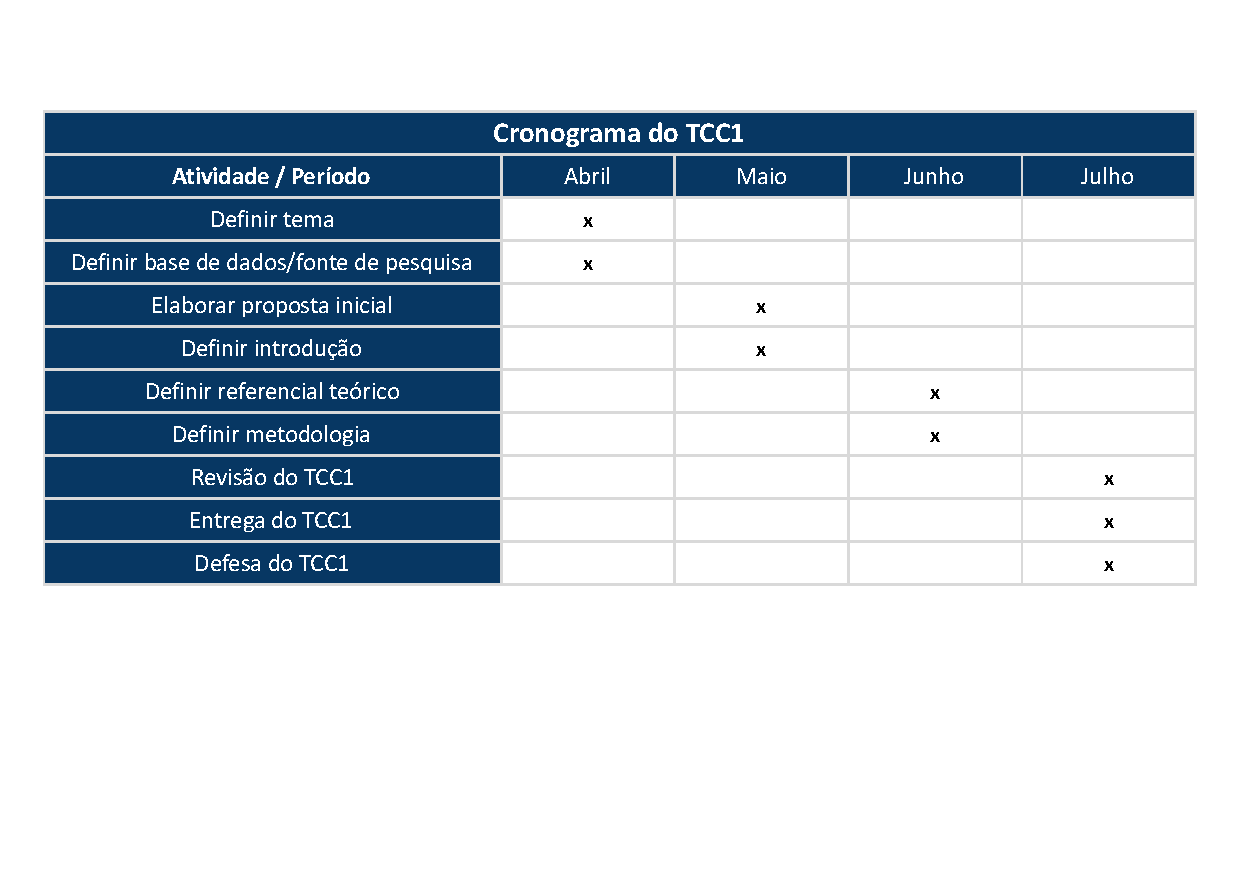
\includegraphics[width=1.0\textwidth]{figuras/cronograma_tcc1.pdf}
    \vspace{-110pt}
    \caption{Cronograma do TCC1.\\
    Fonte: Autores.}
    \label{fig:cronograma_tcc1}
\end{figure}


A Figura \ref{fig:bpmn1} apresenta uma visualização clara dos diferentes estágios do projeto, incluindo as fases de pesquisa, coleta de dados, análise, elaboração da estrutura do trabalho, redação e revisão. Cada marco definido no cronograma representou uma etapa importante do processo de desenvolvimento do TCC1.

\begin{figure}[H]
    \centering
    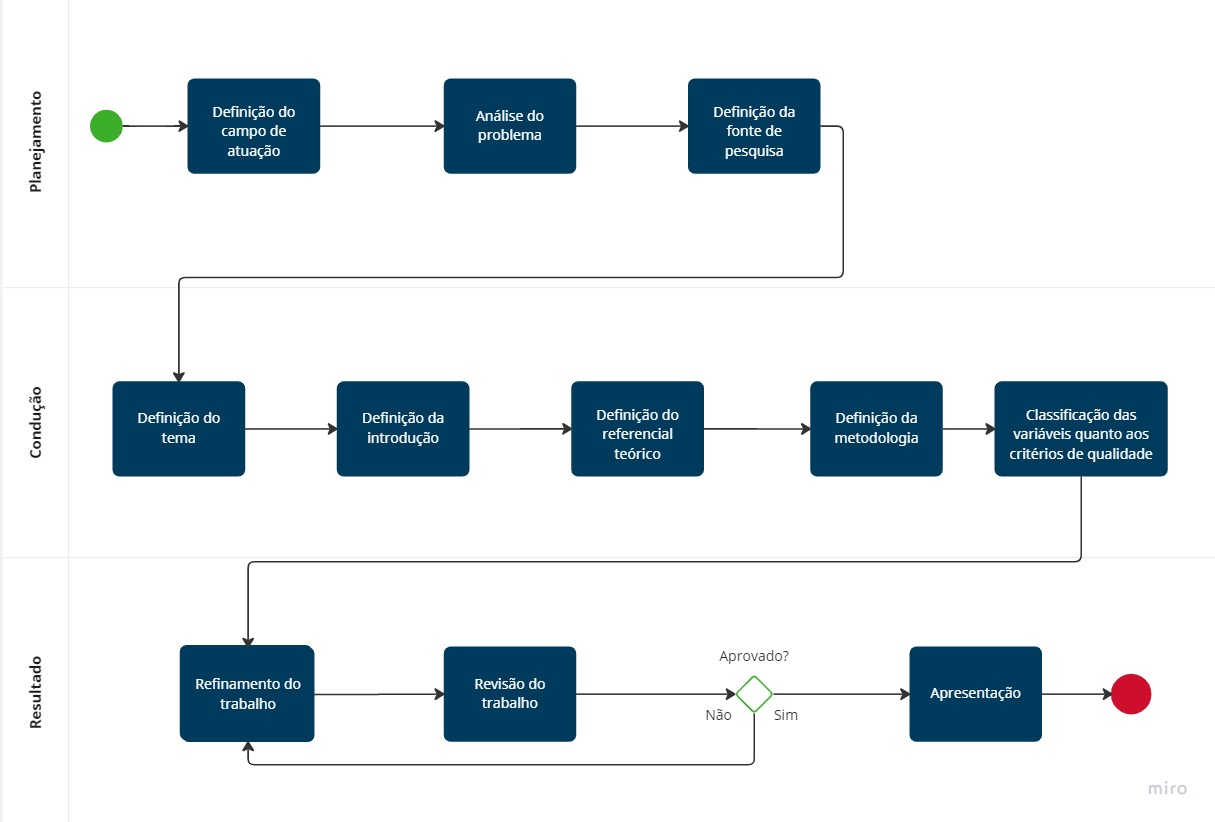
\includegraphics[width=0.8\textwidth]{figuras/bpmn1.jpg}
    \caption{Processo BPMN do TCC1.}
    \small Fonte: Autores.
    \label{fig:bpmn1}
\end{figure}

\subsection{TCC2}

O cronograma a ser seguido no TCC2, apresentado na Figura \ref{fig:cronograma_tcc2}, desempenha um papel essencial na organização e no gerenciamento adequado das etapas do trabalho. Ele tem como objetivo orientar o progresso do projeto, garantindo que todas as atividades necessárias sejam concluídas dentro dos prazos estabelecidos.

\vspace{-40pt}
\begin{figure}[H]
    \centering
    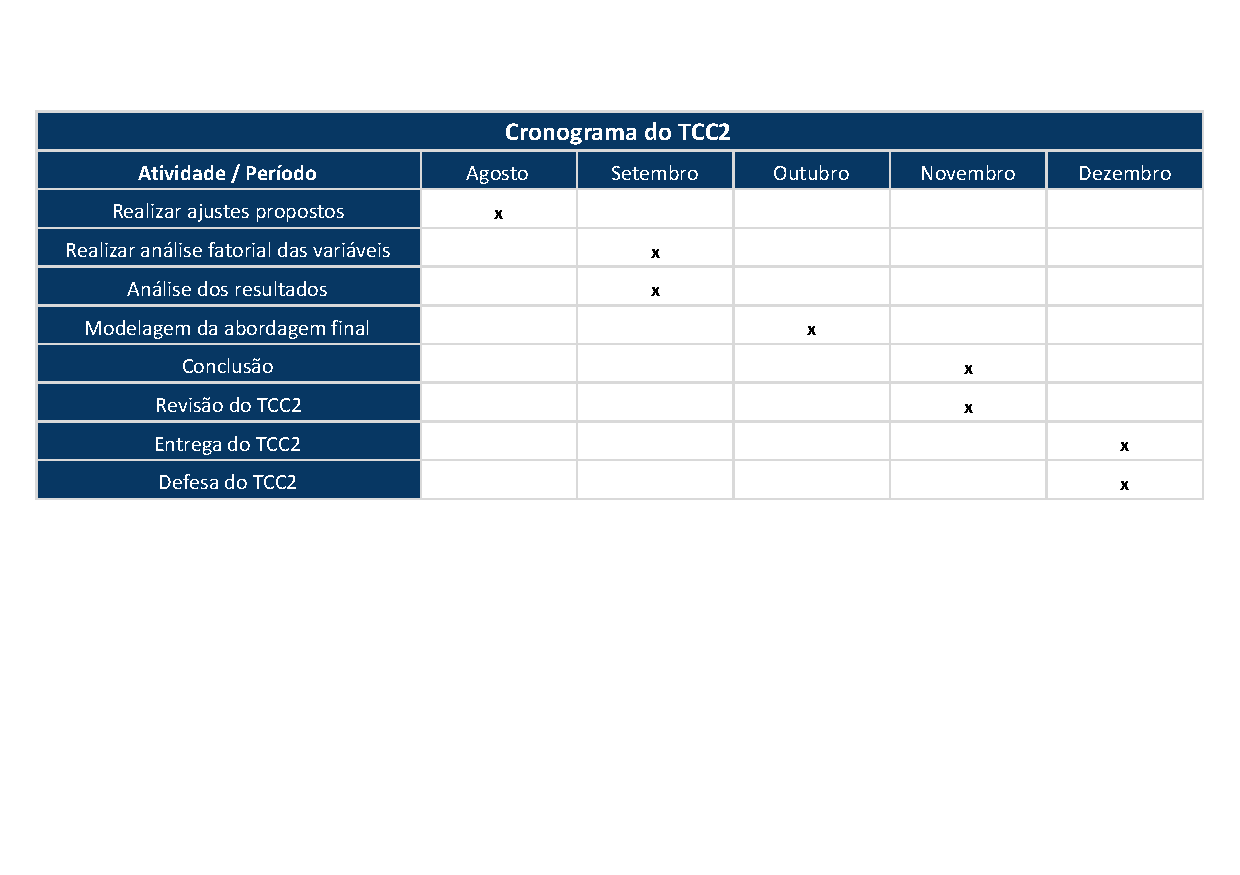
\includegraphics[width=1.0\textwidth]{figuras/cronograma_tcc2.pdf}
    \vspace{-150pt}
    \caption{Cronograma do TCC2.\\
    Fonte: Autores.}
    \label{fig:cronograma_tcc2}
\end{figure}

O processo BPMN do TCC2 representa a sequência de atividades e eventos envolvidos na condução e conclusão bem-sucedida do trabalho de conclusão de curso. Esse processo visa fornecer uma estrutura clara e organizada para orientar as etapas necessárias para a elaboração e apresentação do TCC.

\begin{figure}[H]
    \centering
    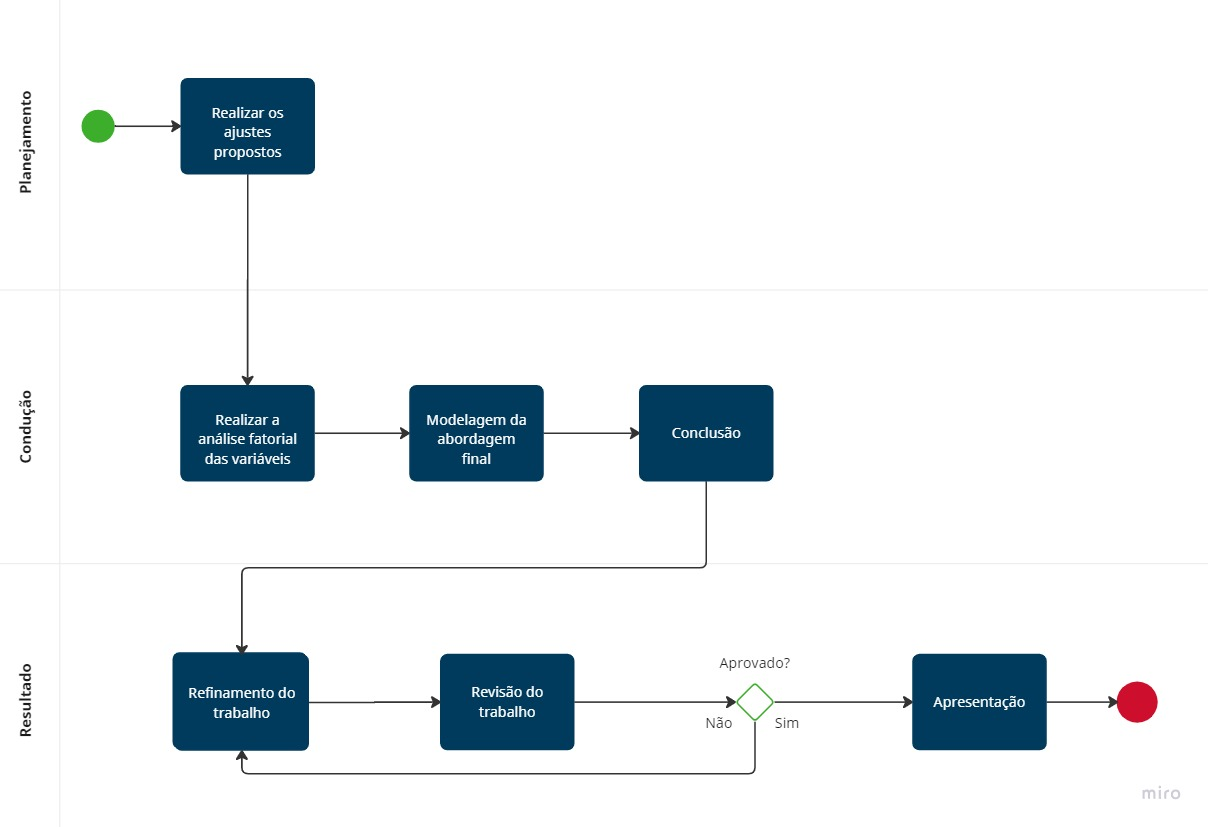
\includegraphics[width=0.8\textwidth]{figuras/bpmn2.jpg}
    \caption{Processo BPMN do TCC2. \\
    Fonte: Autores.}
    \label{fig:bpmn2}
\end{figure}

